
\section{Introduction}

\subsection*{Historical significance}
The established process of trial and error has always underpinned our survival \citep{TrialandError}. Babies are born to rely on a set of sensory reflexes and a framework for physical reasoning \citep{pr}, and with these, we develop methods to navigate the influence of change within a physical, and auditory space \citep{objects}. This method of decision making is reflected in our adult lives with ideas and actions being limited in choice by our intuition and experience \citep{descartes}. In science, we apply a methodological framework consisting of a continuous assessment of scepticism, educated guessing (hypothesising) and rigorous practical testing. Specialists accrue years of practical and theoretical knowledge within a narrow field and can identify areas of potential gain and futility. Yet even with all prior experience, the discovery of new and untested techniques involve the tortuous traipsing through a sea of uncertainty. Such a methods sometimes prove fruitful, through accidental discoveries of items such as x-rays, penicillin... \citep{accidental}; finding novel applications for existing methods such as optical tweezers for chemistry or the abstract field of maths utilised by Einstein [REF], but more often than not end in the constant evolution of a pre-existing project with no apparent result. 

\subsection*{Theory and Simulation in Science}

Until recently much of the experimentation possible was limited by resources, levels of knowledge available technology. With the increase of computation power, we have been able to not only increase our understanding but also run theoretical simulations to guide exploratory efforts with an impact on real-world applications \citep{dft,lion,theoreticalbio,drug}. However, as our ability to record and produce data increases, the need for the scientific method diminishes \citep{wired}. Here the application of `big data' tools and algorithms can provide insights and correlations much more compelling than the predictive capabilities of constantly changing models - ``Since all models are wrong the scientist cannot obtain
a "correct" one by excessive elaboration'' - \cite{allmodels}. As our level of attainable technology increases, so does the complexity of the data collected. New datasets tend to be large, complex and highly multivariate. Although this dramatically improves the quality of science, the difficulty lies in trying to represent it in such a way that we may successfully access the reliability of the results. Since simple bar and line graphs are no longer applicable, one solution falls within a class of unsupervised machine learning techniques called dimensionality reduction (DR).


\subsection*{Chapter Aims}
In \autoref{ch1}, we looked at visual representation as a way of understanding complex systems. \autoref{ch2} showed that the chemical properties could be inferred (visually) from the node-link graph structure of a mechanism. Similarly, \autoref{ch3} and \autoref{ch4} located the presence of important species and clusters of similar properties by applying mathematical algorithms to the graph network. As opposed to attempting to visualise complex data, this chapter looks at learning the structure of a chemical species and simplifying it into two dimensions. Here it is possible to extract key features of like-groups through the use of vector clustering, which unlike the graph clustering in \autoref{ch4} works by determining the density between points on a plane.  

The chapter begins with the introduction of the chemical system, and the various methods for representing species structure within it (\autoref{sec:drinput}). Next, we define the dimensionality reduction methods, which are to be used to simplify the inputs above (\autoref{sec:dr}). This is followed by a brief overview of the visualisation methodology (\autoref{sec:visdr}). Finally, all three sections are combined to produce a set of result and conclusions about the use of DR to identify species structure.  



\section{Species of the MCM and ways to represent them.}\label{sec:drinput}
The master chemical system (as defined in all previous chapters), represents our foremost knowledge of gas-phase chemistry within the troposphere.  \autoref{ch2} shows that information about a species structure is encoded within its reactions, much of which can be attributed to the well-defined construction protocols. 

This section explores the different methods of representing a species structure, intending to provide a machine built algorithm with the highest amount of information about each species and its functionality. A range of input types will be evaluated against several dimensionality reduction algorithms to isolate which chemical properties are most `picked up'. 

\subsection{Input generation}
The MCM provides species information in the form of a species `smiles' (\autoref{sec:smiles}) and the IUPAC InChi string \citep{inchi}. Within this chapter, we use only the smiles string, which is either manually processed using regular expressions or with the aid of pythons RDKIT package \citep{rdkit}. There are seven different methods for representing the chemistry; these are outlined below. 


\subsection{Manual Categorisation}
Reactions within the MCM are determined by a set of rules (PROTOCOL SECTION). These mimic the process a chemist my discover new species and often rely on the bond availability and functionalisation of a species. Since the present functional groups are the benchmark of whether a DR algorithm has successfully separated species structure, it makes sense to run a unit test using the known functional groups of a species as the input. 

To generate the functional groups the regular expressions in \autoref{tab:fngroups} are used\footnote{To see the structure of each functional group type, go to \autoref{appendix:fngroups}.} on the smiles strings (described in \autoref{sec:smiles}) for each species. In extracting the functional groups, we can plot the likeliness a species with a certain group is likely to have another using a chord diagram - \autoref{fig:covermcm}. Since most species contain a multitude of functional groups, the separation of these into `tidy' clustered groups seems unlikely.      


%
% Except for dissociation, species reactions are often dictated by their functional groups. Species in the MCM are usually represented as functionalised alkanes (A saturated hydrocarbon in the form of $C_nH_{2n+2}$). In removing hydrogen, we form an alkyl chain. This allows for the potential of forming a bond with other atoms. By themselves alkyl chains are mostly un-reactive, however in gaining additional functional groups (functionalisation) their reactivity increases.%



\begin{table}[H]
    \centering
    \begin{tabular}{c|p{5in}}


PAN & \verb! C\\(=O\\)OON\\(=O\\)=O$|^\\[O-{0,1}\\]\\[N\\+{0,1}\\]\\(=O\\)OOC|!\\&\verb! O=N\\(=O\\)OOC\\(=O\\)|C\\(=O\\)OO\\[N\\+{0,1}\\]\\(=O\\)\\[O-{0,1}\\]!\\&\\

Carb. Acid & \verb! [^O](C\\(=O\\)O$|^OC\\(=O\\))!\\&\\

Ester & \verb! [\^O](C\(=O\)O\b|OC\(=O\))C!\\&\\

Ether & \verb! (\([\^O=]+\))*C(\([\^O=]+\))*O(\([\^O=]+\))*C(\([\^O=]+\))*!\\&\\

Per. Acid & \verb! c\\(=O\\)OO$|^OO\\(=O\\)C!\\&\\

% Hydroperoxide & \verb! COO$|C\\(OO|OO\\)C|^OOC!\\&\\

Nitrate & \verb! O(NO2\b|NOO\b|N\(=O\)=O|\[N\+\](?:\[O-\\]|\(=O\)){2})!\\&\\

Aldehyde & \verb! C=O$|^O=C!\\&\\

Ketone & \verb! C\(=O\)C!\\&\\

Alcohol & \verb-CO\\b|(?=^\\b)(?!^\\[)CO.|(?=^\\b)(?!^\\[)OC.|\\(O\\)|C\\)O(\\b|[^O]-\\&\\

Criegee & \verb! \[O-\]\[O\+\]!\\&\\

Alkoxy rad & \verb!\[[\/]{0,1}CH{0,1}\]|\b[\^O]\[O\.{0,1}\]!\\&\\

Peroxyacyl rad & \verb! \\ w\(=O\)O\[O\.{0,1}\]!\\&\\

    \end{tabular}

    \caption{CHECKKKKKKK!!!!!!!!!  A set of regular expressions that may be used to determine the number of occurrences of a functional group within a SMILES string.}
    \label{tab:fngroups}
\end{table}



\begin{figure}[H]
    \centering
    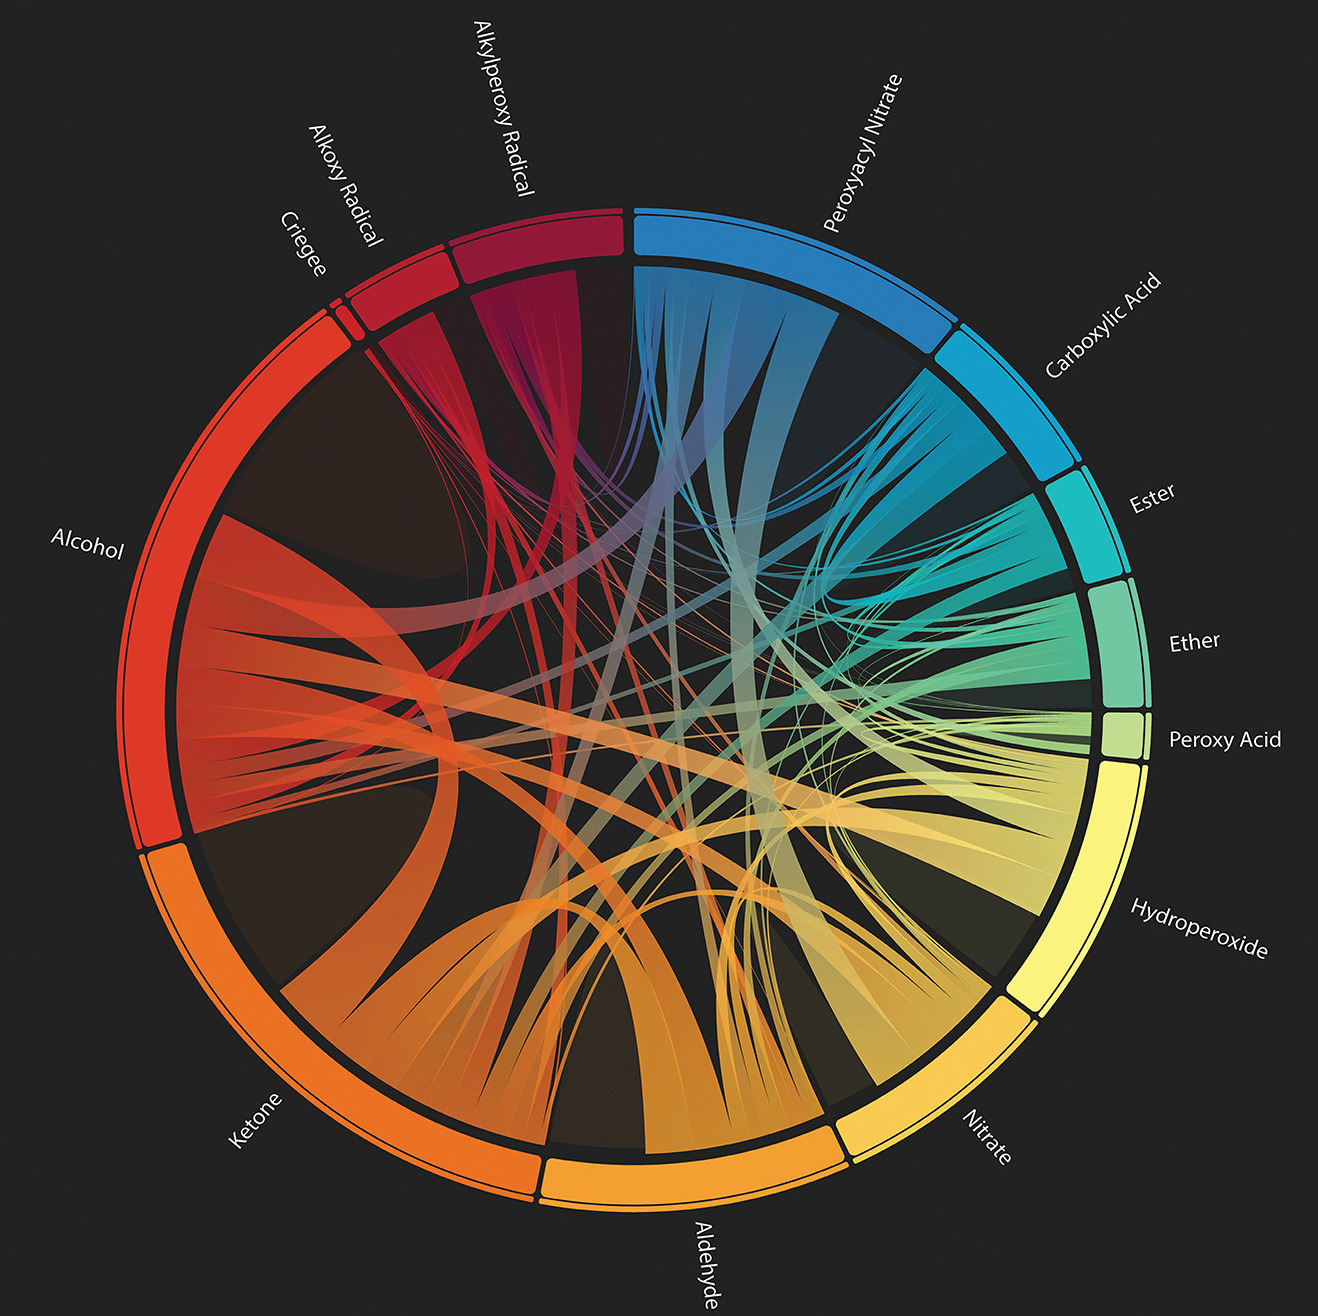
\includegraphics[width=\textwidth]{4fig/coverfig.jpg}
    \caption{\textbf{The multifunctionality of the MCM.} A chord diagram showing the functionalisation of a species within the MCM. Arc sizes represent what percentage of all functional groups in the MCM mechanism a group contains. Translucent areas of no outwards links represent species with multiples of a certain functional group, of which Alcohols and Ketones have the most.  
    Source: \citep{cover} }
    \label{fig:covermcm}
\end{figure}



\subsection{Tokenization}
As computer algorithms are unable to understand words or their meaning, we have to first categorise the data into groups. Tokenisation is the conversion of a string into characters and representing them with a numerical equivalent. In doing so, a string of characters can be converted into a numerical vector, allowing for its representation in a latent vector space. 
Within our input selection, we have two sets of inputs we can convert. These are the species names, and their smiles string representation. 



\subsubsection{Species Names}
In \autoref{ch4} it was shown that the dedicated species names for species in the CRI mechanism were often representative of their structural properties. This adage also applies for the MCM, where an intuitive naming convention is used. This is often derived as part of the construction protocol, where a species names reflect its own, or its precursor's structure (which it will have at least in-part inherited).

Although this is not the most robust method of defining the structure, it allows for a straightforward test of the algorithms, for which the user can quickly compare the human-readable output. 


\subsubsection{SMILES strings}\label{sec:smiles}


 Smiles (`Simplified Molecular-Input Line-Entry System') provide a human-readable representation of the molecular structure,
 \citep{smiles}. They offer a linear human-readable description of the chemical composition within a molecule - making it easy to visually check the construction of a species without any additional work. Besides, their role in generating the molecular fingerprints in \autoref{sec:fingerprints} makes it a useful comparison to make when evaluating methods of structure representation. 

\paragraph*{Construction Methodology of SMILES strings}
The construction of a SMILES string happens in three parts:

\begin{enumerate}
    \item The smiles string is built by creating the longest possible chain to form a molecule backbone.
    \autoref{fig:st2}

    \item This may within itself contain aromatic rings denoted by the lowercase carbons and a number corresponding to the location of each break cycle. \autoref{fig:st3}

    \item Finally all the functional groups and branches attached to the main backbone are added. These are nested within the parenthesis to show that they are not part of the skeletal backbone. \autoref{fig:st4}
\end{enumerate}



\begin{figure}[H]
     \centering
     \begin{subfigure}[b]{0.495\textwidth}
         \centering
         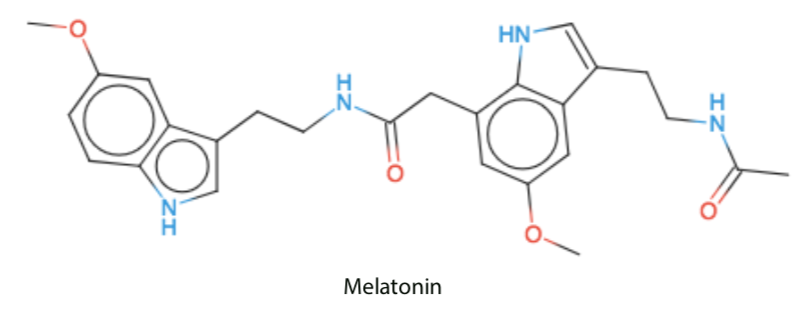
\includegraphics[width=\textwidth]{4fig/sm4.png}
         \caption{Structure of Melatonin}
         \label{fig:st1}
     \end{subfigure}
     \hfill
     \begin{subfigure}[b]{0.495\textwidth}
         \centering
         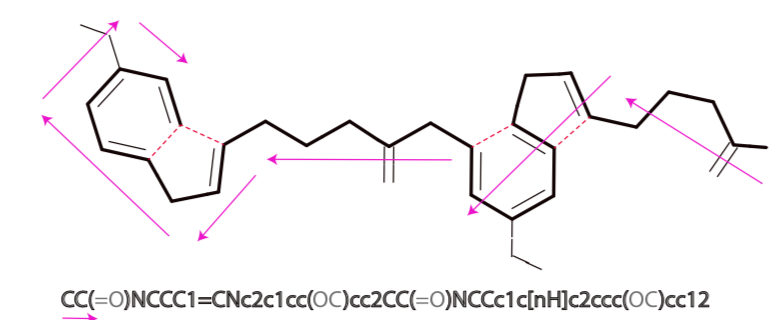
\includegraphics[width=\textwidth]{4fig/sm1.png}
         \caption{Step 1 : Building the C chain backbone.}
         \label{fig:st2}
     \end{subfigure}\\

     \begin{subfigure}[b]{0.495\textwidth}
         \centering
         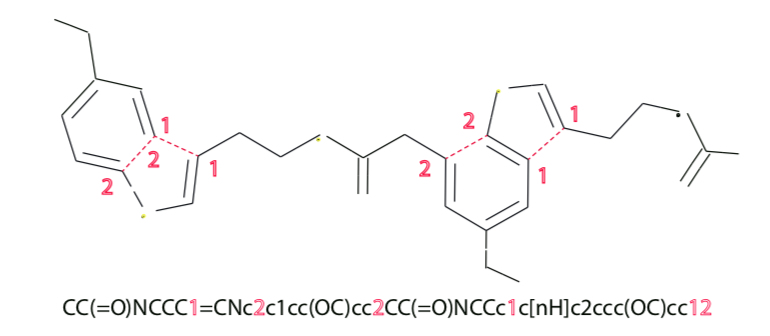
\includegraphics[width=\textwidth]{4fig/sm3.png}
         \caption{Step 2 : Aromatic Rings}
         \label{fig:st3}
     \end{subfigure}
     \hfill
     \begin{subfigure}[b]{0.495\textwidth}
        \centering
            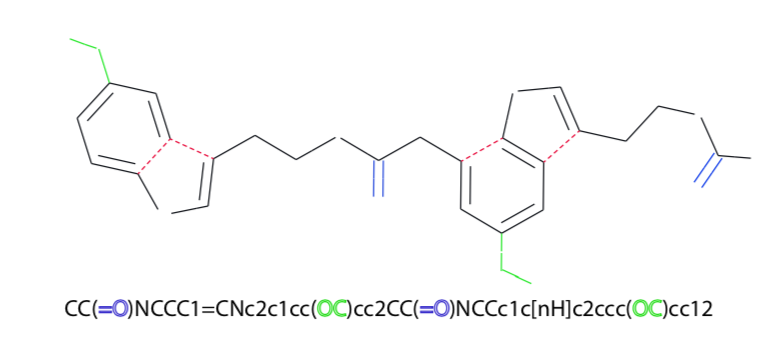
\includegraphics[width=\textwidth]{4fig/sm2.png}
            \caption{Step 3 : Functional Groups }
            \label{fig:st4}
        \end{subfigure}

        \caption{ \textbf{Construction process of a smiles string.} The example compound is Melatonin. Although this does not exist within the atmosphere, it provides a clear example of the smiles string methodology. \autoref{fig:st1} is made using smiles drawer: \citep{smilesdrawer} }
        \label{fig:smiles}
\end{figure}


\subsection{Graph Inspired}

\autoref{ch2} - \ref{ch4} have shown the role of graphs in revealing network properties and structure. Graphs in themselves can simplify relational data into two/three dimensions for visualisation and algorithmic clustering. Continuing this trend, we can represent a species structure in the form of a graph (\autoref{sec:specgraph}), as well as converting the structure of a mechanism for dimensionality reduction (\autoref{sec:n2vec})


\subsubsection{The species graph (fingerprint)}\label{sec:specgraph}

The structure of a species has long represented using a graph-like layout, \autoref{ch2}. It, therefore, follows that other methods for representing the graph structure would also apply. One such way is the use of an adjacency (or relational) matrix to describe the relationships between atoms and bonds in a species. Such a methodology is already used in the construction of bond and z-matrixes \citep{mcmgen,zmatrix}. 

The construction of a structure matrix/graph begins with a chemical species. Here the relationships between atoms (\autoref{fig:graphmol}) is converted into an adjacency matrix (\autoref{fig:adjmol}). However, since species have different numbers of each atom, a template allowing us to compare different graphs is required. To do this a maximum occurrence table (\autoref{table:my_maxoccur}) is created. Here, for example, BCARY \ch{C15H24}, a sesquiterpene contains the most carbon atoms of any species within the MCM. This universal matrix is now able to contain any possible combination of atoms in a species. 

As machine learning algorithms only vectors as an input, it is possible to decompose the $37^2$ element adjacency matrix into rows, which can then be joined together, Using this method we create a one-dimensional array (vector) of 259 elements (518 bytes) to represent our species.


\begin{figure}[H]
     \centering
     \begin{subfigure}[b]{0.325\textwidth}
         \centering
         \begin{tabular}{c|c}
         \textbf{Atom} & \textbf{Max}\\
         \hline\hline
         &\\
             C & 15 \\
             Cl & 4 \\
             O & 12\\
             N&3\\
             S&1\\
             BR&2\\
         \end{tabular}
          \caption{}
         \label{table:my_maxoccur}
     \end{subfigure}
     \begin{subfigure}[b]{0.325\textwidth}
         \centering
         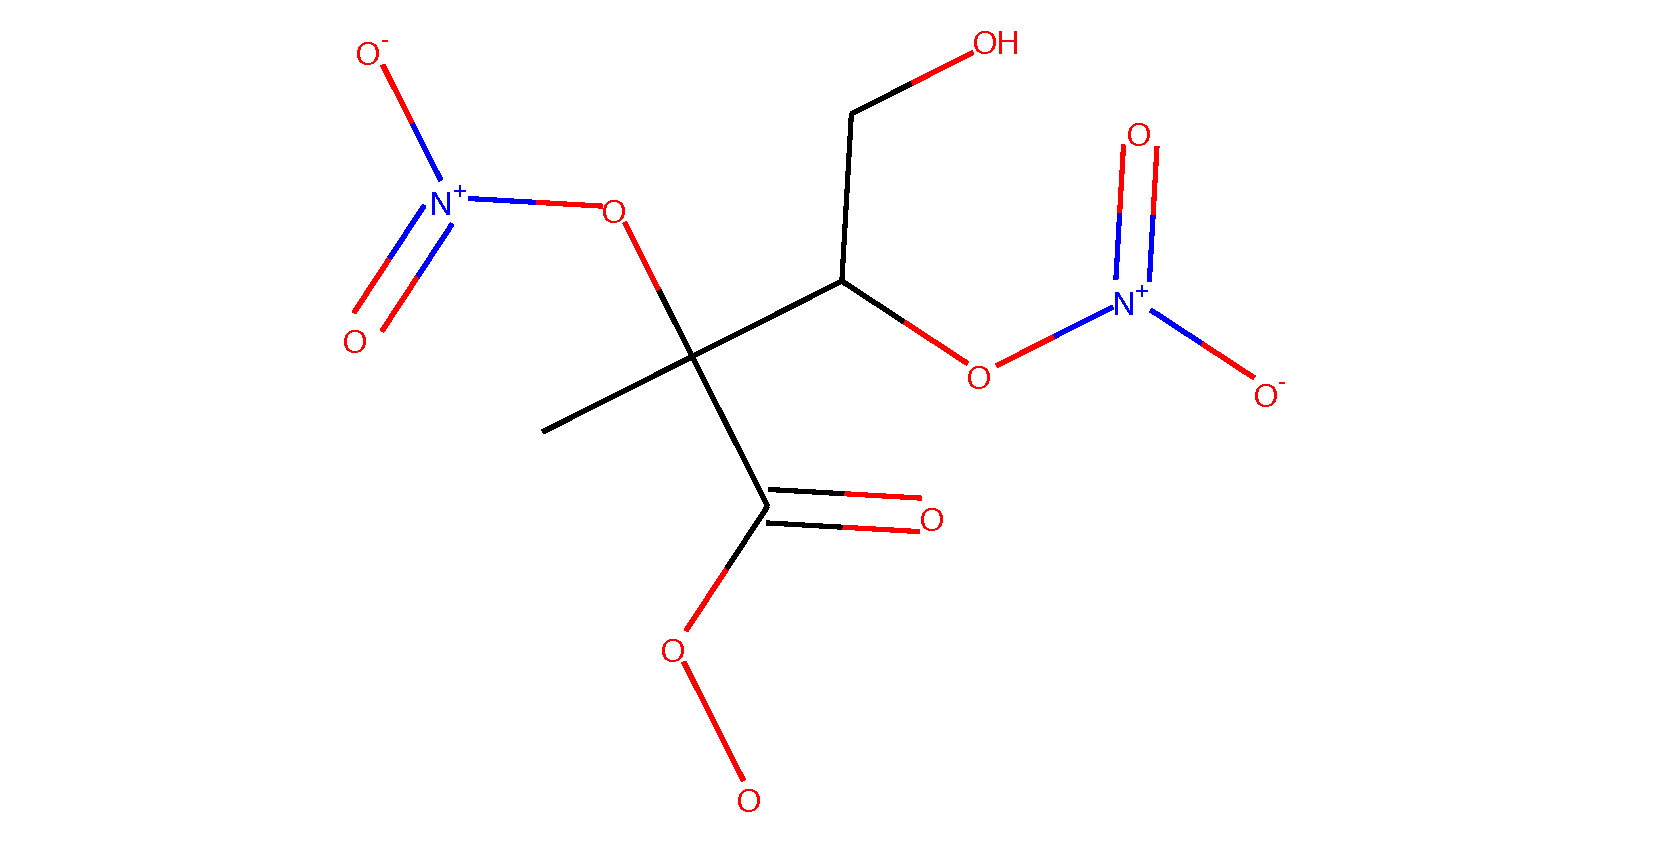
\includegraphics[width=\textwidth,height=.8\textwidth]{4fig/INB1NBCO3.pdf}
         \caption{}
         \label{fig:graphmol}
     \end{subfigure}
     \hfill
     \begin{subfigure}[b]{0.325\textwidth}
         \centering
         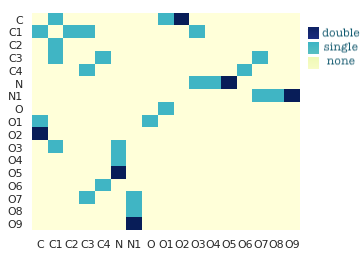
\includegraphics[width=\textwidth,height=.8\textwidth]{4fig/INB1NBCO3_adj.png}
          \caption{}
         \label{fig:adjmol}
     \end{subfigure}

        \caption{ \textbf{Constructing a graph from species structure.} 
        (a) shows the maximum number of times an atom occurs for any single species in the MCM. (b) depicts the graph-like chemical structure of \ce{INB1NBCO3}. This is a highly processed species stemming from Isoprene, and this makes for a good example of the bond matrix. Finally, a matrix representing the bonds in \ce{INB1NBCO3} is created from the maximum possible occurrence matrix from (a). For simplicity, empty row/column pairs have been removed to produce (c). This matrix will always be symmetrical as the bonds do not have a direction.}
        \label{fig:bondmat}
\end{figure}


\subsubsection{Node Embeddings (node2vec)}\label{sec:n2vec}
\autoref{ch2} and \autoref{ch3} showed that the underlying structure of a chemistry mechanism graph contains information about the species and reactions within it. In \autoref{fig:vk} colour represents the ratio of potential oxidation of a species. Here as emitted species become progressively more processed, the number of bonds which may be oxidised diminishes (lighter colours near the centre) until they eventually form carbon dioxide and water. 


\begin{figure}[H]
  \centering
  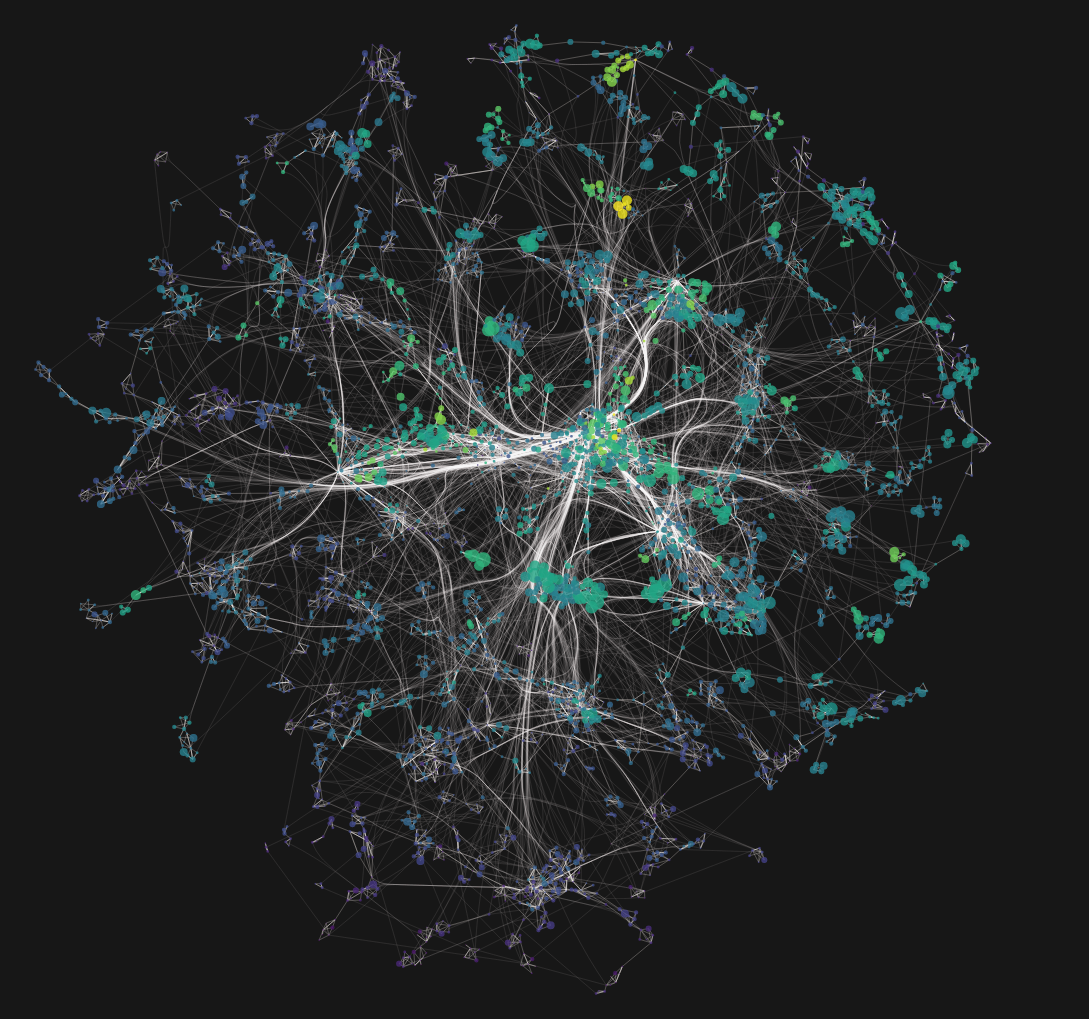
\includegraphics[width=\textwidth]{4fig/graph/oxidised_ratio.png}
  \caption{\textbf{The graph of an MCM subset representing the chemistry within Beijing.} Here colours show the increase of \ce{O-C} ratio as species are oxidised (lighter). All emitted species ultimately tend towards carbon monoxide which is at the centre of the graph. }
  \label{fig:vk}
\end{figure}

This type of structural information can be extracted through the use of a natural language processing package capable of transforming a graph into a vector - node2vec \citep{node2vec}. Since this may also be used for dimensionality reduction, it is described within the next section (\autoref{sec:n2v}).




\subsection{Molecular Fingerprints}\label{sec:fingerprints}

In the field of chemical informatics, molecular fingerprints (or structural keys) are used to encode and query structural properties of species. Their binary representation makes them suitable for dimensionality reduction and the exploration of fo chemical space (a type of property space constructed using pre-determined features and boundary conditions).

Here species properties are often split into structural and psyico-chemical groups - which has used such as the discovery of natural analogues (which circumvent problems such as intolerances in medicine \citep{analog}). Although there exist many different types of molecular fingerprints, the two main ones that will be explored are molecular quantum numbers (MQN) and the molecular access system (MACCS). 

\subsubsection{Molecular Quantum Numbers (MQN)}
In chemistry the shape, phase and electron occupancy of an atom may be described through the use of four quantum numbers: the $n$ principle quantum number, $I$ angular momentum quantum number, $M_i$ magnetic quantum number and $M_s$ spin quantum number. The rationalisation of elements based on their structure, and by consequence reactivity, has led to the most iconic tool of the modern-day chemist - the periodic table, where increasing atomic numbers follow the principal quantum number \citep{periodic}. In representing a molecule as a set of 42 quantum numbers, MQN fingerprints produce a multi-dimensional mapping of atom, bond, polarity and topology count \citep{MQN}. 

% [ref fae others... ]

\subsubsection{Molecular ACCess System (MACCS)}
MACCS keys are a 164\footnote{They are 166-bit keys, although there is no real agreement to what the 44th keys' purpose is, and therefore it is often omitted. Within RDKIT this is denoted by a $?$ \citep{rdkitcode}.} bit structural keys formulated through answering a series of structure-related questions. Developed by MDL Information Systems \citep{maccs}, their main purpose lies in being a SMILES Arbitrary Target Specification (SMARTS) system for substructure searching. However, their distinct structure key format makes them highly suitable for similarity detection. In many cases, the optimised version of MACCS keys is cited (\citep{optimised}), although most use cases exploit a variation of the undocumented 166bit keys. We use the implementation presented by \citep{rdkit,rdkitcode} for all molecular fingerprints in this section.


\section{ Dimensionality Reduction Methods}
In the last section, we described several methods in which the chemical structure of a species could be encoded for direct comparison. However, since each input consists of a multitude of elements, it is still not a simple task to determine the differences and similarity between all species in mechanisms. Dimensionality reduction is the process of reducing the number of random variables and only presented a set of principal values, by mapping a high-dimensional space into a low-dimensional one \citep{drrandom}. This allows us to flatten a multivariate input into the two dimensions required for a simple scatter plot.

In this section, we begin by explaining the data preparation required for dimensionality reduction (\autoref{sec:pref}) before describing the different possible methods of reducing the dimensions of a dataset. 

\subsection{Preperation of the data}\label{sec:prep}
Real-world data is rarely preformatted in such a way that it can be used directly within a computational model. Often values need to be cleaned and corrected to be fit for purpose. In the interest of completeness, the two main methods of data adjustment for machine learning are outlined below. These are normalisation and standardisation. 


\subsubsection*{Normalisation}
In the data is without (dimensionless) or of a single unit, it is possible to rescale the data between a range - most commonly {0,1}. In doing so it is possible to interpret the importance of value in contrast to the largest recorded value. This gives us a percentage scale spanning the range of the data. Such a range is useful in the definition of colourmaps and describing the importance of value relative to the dataset. 
To rescale a dataset we shift the minimum value to zero, then divide by the new maximum of the dataset (Note this is equivalent to the range of the unshifted dataset.)

\begin{equation}
    n(x_i) = \frac{x_i - \min_x }{\max_x - \min_x}
    \label{eqn:n}
\end{equation}



\subsubsection*{Standardisation}
If the components we wish to compare are of different units or are expressed with a different scale, normalising them would not produce meaningful data. Instead, it is possible to standardise the data by looking at each points deviation from the mean. Here the variation of the mean for a dataset is divided by the standard deviation to produce a value between \{-1,1\}, \autoref{eqn:z}. In statistics this is known as the `z-score'\footnote{Possibly because of the American spelling of standardi\textbf{Z}ation?}

\begin{equation}
    z(x_i) = \frac{x_i - \mu_x}{S}
    \label{eqn:z}
\end{equation}\\    


\subsection{Principle Component Analysis}
One of the most well-known dimensionality reduction methods is the determination of the principal components through the use of Principal Component Analysis (PCA). PCA increases the readability of a dataset by creating a set of new uncorrelated variables which maximise the variance \citep{pcareview}. 


 PCA works on the assumption that components within a dataset are linear combinations of each other. By simplifying these linear combinations, it is possible to identify the elements which explain the most variability in a dataset - these are the principal components. 

A more straightforward interpretation of this would be to adjust the direction of each axis of the data, such that its projection has the most prominent variability. In doing so, it is possible to determine which components contribute the most to changes in the dataset \citep{pca,pca2}. An example of this is seen in \autoref{fig:2dpca}, where the second component of the original data can be removed with little effect on the overall result of the data. Such methods have applications in compression and signal filtering \citep{pcacompress,pcanoise}.


\begin{figure}[H]
    \centering
    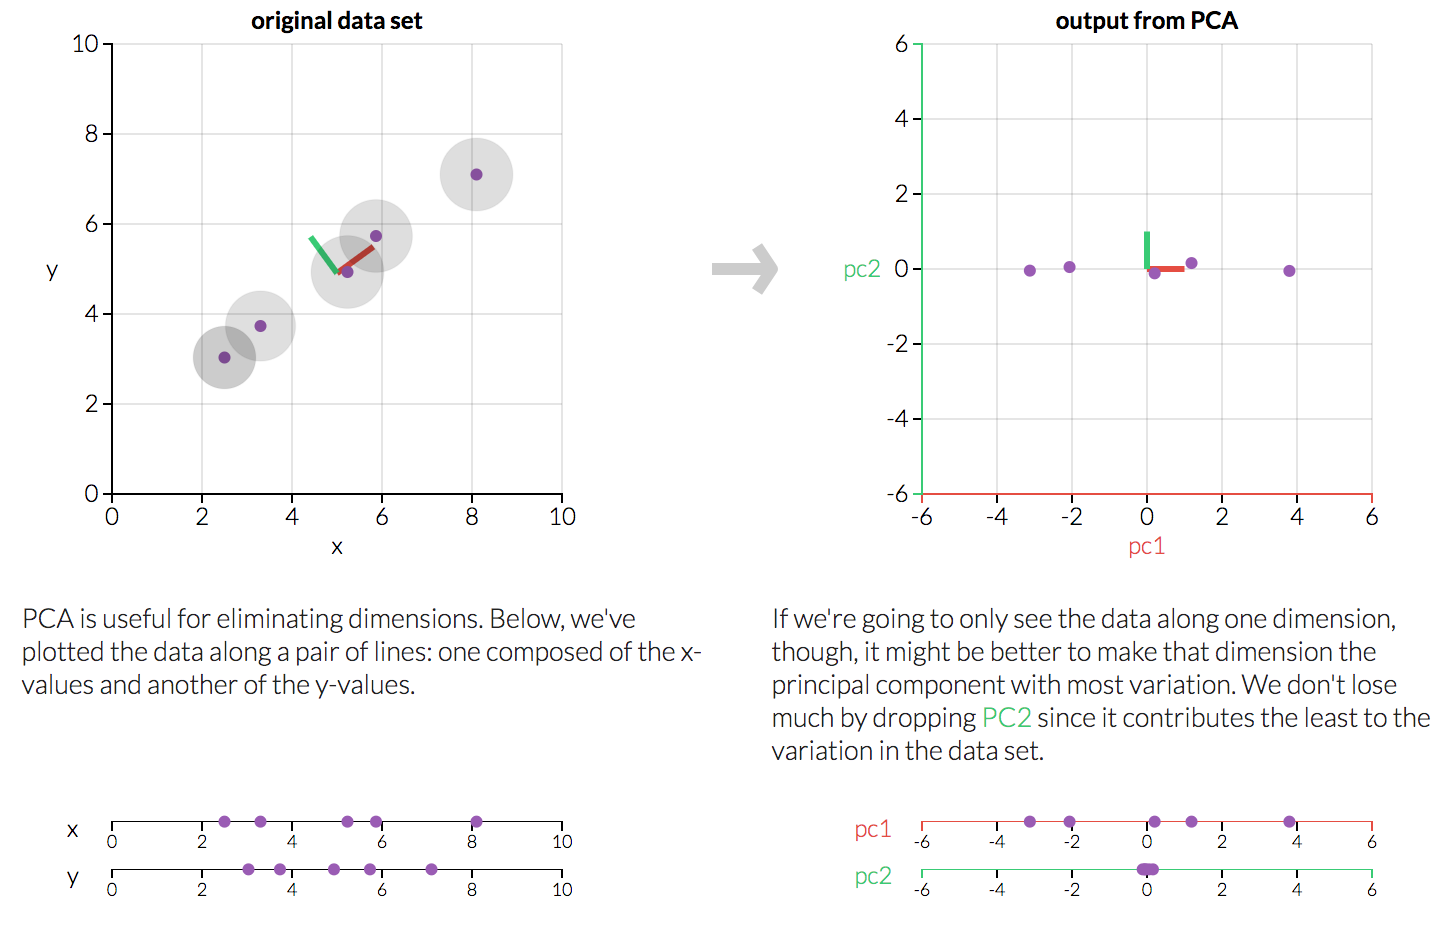
\includegraphics[width=.8\textwidth]{./4fig/pca2d.png}
    \caption{\textbf{Determining the Principal Compnent of a sample dataset.} It can be seen that in a change in axis to follow the first principal component (right), it is possible to explain most of the variation in the samle dataset (left). Source: \citep{pcaim}}
    \label{fig:2dpca}
\end{figure}


\subsubsection{Mathematical explanation of PCA}
\emph{\textbf{Note:} The basic statistics/mathematics required to understand this section is shown in \autoref{apendix:pca}. Please read this if you are not familiar with any of the terms below.
}

The mathematics behind PCA consists of first calculating the covariance matrix - an $n \times n$ matrix outlining how strongly each variable changes with every other. Using this we can calculate both the eigenvalues and eigenvectors of the matrix \footnote{These need to be unit vectors, although most packages already do this out of the box.}. This can be done using a computational package such as numpy or scipy \citep{numpy,scipy}.

We can now sort the eigenvector columns by influence using their eigenvalues—this way a feature dataset can be produced by removing vectors of low importance. The final feature dataset can now be transposed and multiplied by the transpose of the original dataset. This results in an output dataset containing each principal component of the desired dimension.



\subsection{t-Distributed Stochastic Neighbor Embedding (t-SNE)}\label{sec:overcrowd}

t-SNE is an algorithm designed with visualisation in mind \citep{tsne}. Rather than representing the data through a series of linear transformations, t-SNE uses local relationships to create a low-dimensional mapping, much in the same way as a fully connected force graph, \autoref{fig:tsneforcegraph}. This allows the ability to capture non-linear structures in the data which cannot be accomplished through linear mapping methods (e.g. PCA).

\begin{figure}[H]
    \centering
    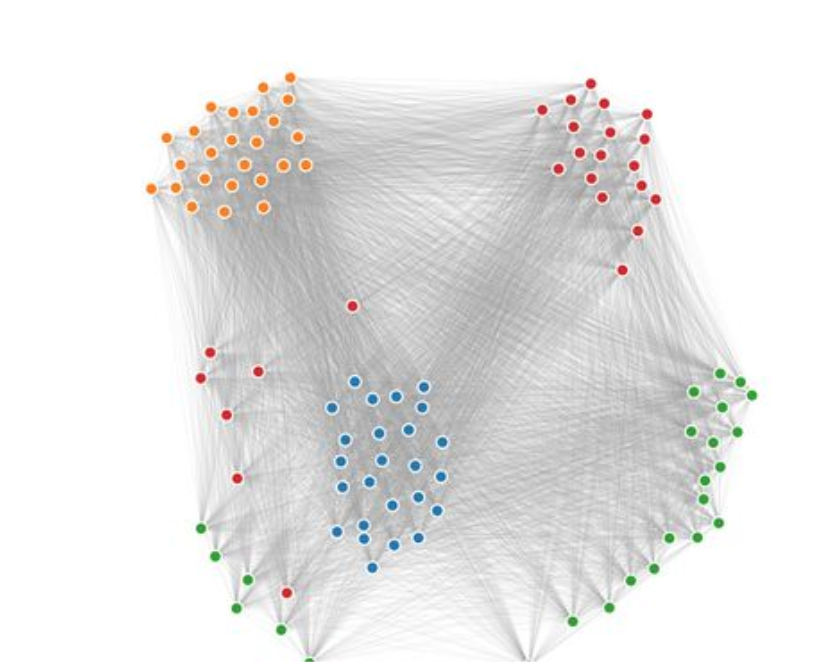
\includegraphics[width=.6\textwidth]{./4fig/tsneforcegraph.png}
    \caption{\textbf{Representing the t-SNE algorithm as a fully connected force graph.} Here each node is attached to every other node. Nodes with a strong relationship are pulled closer together than those with a weaker one.}
    \label{fig:tsneforcegraph}
\end{figure}



The algorithm itself can be simplified into two parts,

\begin{itemize}
  \item [1.] Create a probability distribution which dictates relationships between neighbouring points
  \item [2.] Recreate a lower-dimensional space following the probability distribution established in 1.
\end{itemize}

and is described in \autoref{sec:mathtsne}.The main reason t-SNE produces good results is that it can handle the \textbf{`crowding problem'} very well. The crowding problem is a product of the `curse of dimensionality'. In a high dimensional space, the surface of a sphere will grow much quicker than one in a lower dimension space. This means that the higher dimension spaces will have more points at a medium distance from a certain point, \autoref{fig:dimcurse}. When we map our data into a lower dimension, data will try to gather at its medium distance, resulting in a more `squashed', and thus crowded, output.



\begin{figure}[H]
  \centering
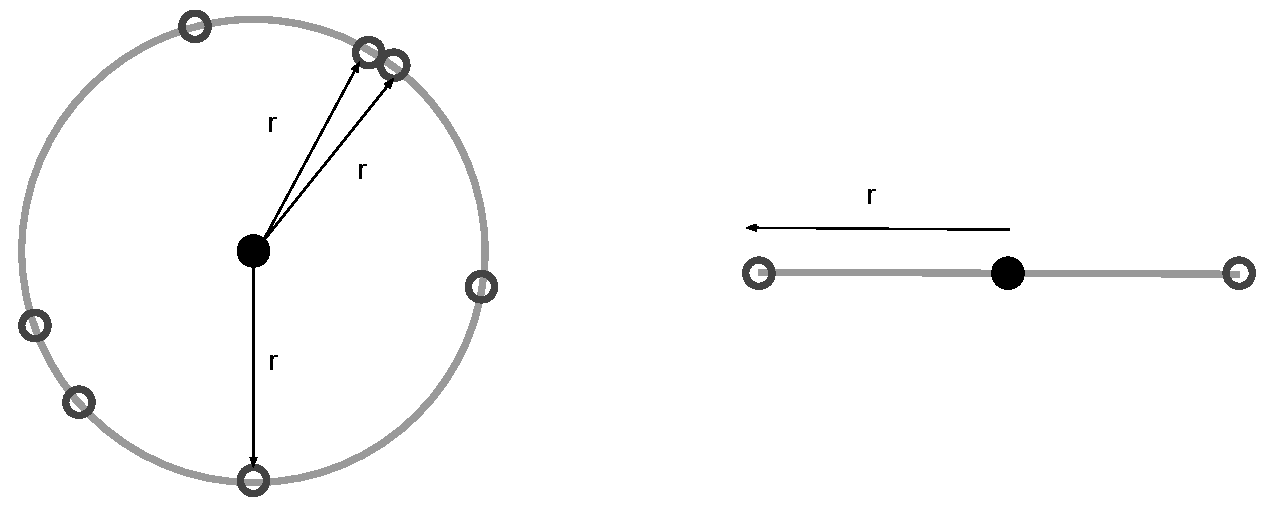
\includegraphics[width=.5\textwidth]{4fig/dimcurse.pdf}
\caption{\textbf{An example of how the curse of dimensionality affects the mapping of points a certian distance from eachother.} }\label{fig:dimcurse}
\end{figure}




\subsubsection{Mathematical explanation of t-SNE}\label{sec:mathtsne}
%https://mlexplained.com/2018/09/14/paper-dissected-visualizing-data-using-t-sne-explained/

%
% The general process is given by the etymological dissection of the acronym, with `t'  standing for the student T probability distribution and S, N (stochastic and neighbour) explaining the use of the distribution across neighbouring points in space.

In the original paper \citep{tsne}, the algorithm is described using the etymologic dissection of its name.

\paragraph{Step 1}
First we begin with Stochastic Neigbour Embedding (SNE) - the distribution across neignbouring datapoints in our high dimension space. This is done by converting the high dimensional Euclidian distances between points into conditional probabilities representing their similarity:

\begin{equation}
p_{ij} = \frac{\exp(-\left \| x_i - x_j \right \|^2 / 2\sigma_i^2)}{\sum_{k \neq l} \exp(- \left \| x_k - x_l \right \|^2 / 2\sigma_i^2)}
\end{equation}

Here $p_{i|j}$ is the conditional probability that $x_i$ may pick $x_j$ as a neigbour. This is proportional to the probability density of a Gaussian $\sigma_i$ centered at $x_i$.

\subparagraph{Perplexity}
Since we want the number of neighbours of each point to be similar in number and prevent a single point from having a disproportionate influence on the entire system we introduce a hyperparameter named \emph{perplexity}. Perplexity works by ensuring that $\sigma_i$ is small for points in densely populated areas and large for spare ones and can be thought of as a scale of the number of neighbours considered for any one point in the system. Generally, values between 5 and 50 are considered to give good results, with larger perplexities taking global features into account, and by consequence smaller ones, local features.

\paragraph{Step 2}
Now a probability distribution describing the relationship between points has been formulated, we wish to express this as a low dimensional mapping of our inputs $X$ in terms of our output dimensions $Y$. Naturally, we would want to make the low dimensional mapping represent a similar (Gaussian) distribution as in Step 1. However, it often causes issues presented by the `overcrowding problem', \autoref{sec:overcrowd}, as the gaussian has a `short tail', and thus nearby points are likely to be pushed together. A solution to this is the student t-distribution which has a longer tail \footnote{The distribution employed is a t-distribution with only one degree of freedom and is identical to the Cauchy distribution}:

\begin{equation}
q_{i|j} =\frac{(1 + \left \| y_i - y_j \right \|^2 )^{-1}}{\sum_{k \neq l} (1 + \left \| y_k - y_l \right \|^2 )^{-1} }
\end{equation}

\emph{\textbf{Note:} The definition and explination of the Student t-distribution is given in \autoref{apendix:tsne}.
}

The optimisation of this equation is achieved through the use of \emph{gradient decent}\footnote{\textbf{Gradient Decent} - an optimisation algorithm used to minimise a function by iteratively moving in the direction of the steepest descent. Gradient descent is used to find local minima and is defined by the negative of the gradient of the system. Its primary usage in machine learning is the updating of parameters (coefficients in linear regression and weight in neural networks).}
 on the Kullback-Leibler divergence \autoref{appendix:kl} between distributions $p$ and $q$. Here the gradient is used to apply an attractive and repulsive force on the items\footnote{A positive gradient signifies attraction, while a negative one corresponds to repulsion.}.




\subsection{PCA vs t-SNE, a quick comparison.}

PCA has been around for much longer than t-SNE, and its uses are well established within the scientific community - an example of this would be the use of sensitivity analysis within mechanism reduction \citep{kinetics}. It is fast, simple and easy to use and very intuitive. The PCA algorithm works by creating a lower-dimensional embedding which best preserves the overall variance of the dataset. Clusters created from the algorithm are grouped in ways, such that they retain the highest variance of the data.

The main drawback of PCA is that it is a linear projection. If our data happened to be in a `swiss roll' (spiral) pattern, we would not be able to `unroll' it. The reason for this is that the PCA algorithm works by viewing the data from different perspectives, much like casting a shadow from various directions. With such an example, there is no one way we can do this that unfurls the spiral.

t-SNE, on the other hand, is a relatively new method \citep{tsne}. Its greatest asset is that linear projections do not limit it. Although more computationally intensive for large datasets, t-SNE produces visibly cleaner results. Unlike in PCA, t-SNE cannot be trained on additional data at a later point; however, the output clusters are more visually distinct (they have less of an overlap). Much like in a force graph, the output from t-SNE is scale-invariant. This means that while the location of clusters in a PCA reduced representation has an attributable quality, those produced by t-SNE will not necessarily contain the same information.

A box model run representative of the chemistry within Beijing was used to compare the differences between PCA and t-SNE. The aim is to classify the diurnal profiles of each species concentration (much like the cosine similarity in \autoref{sec:cosine}). 
Diurnal profiles were extracted on the third day of a spun up model initialised with initial conditions representative of the chemistry within the Beijing environment (\autoref{tab:icsmetric}).
These were then standardised and converted into temporal vectors for use in the algorithms.

\autoref{fig:threegraphs} shows the output of both dimensionality reduction algorithms on the dataset. Different colours represent the location of clusters of similar diurnal profiles. A higher dispersion between clusters and species overlap is seen within the PCA output, \autoref{fig:pcac}. This makes it harder to distinguish species from each other or other groups around them.
Since the distance between clusters within t-SNE does not hold the same mathematical meaning as PCA, the algorithm can provide a better distribution of points, creating better-defined clusters, \autoref{fig:tsnec}. The concentration profile shapes for each coloured group is shown in \autoref{fig:tco}. 


\begin{figure}[H]
     \centering
     \begin{subfigure}[b]{0.495\textwidth}
         \centering
         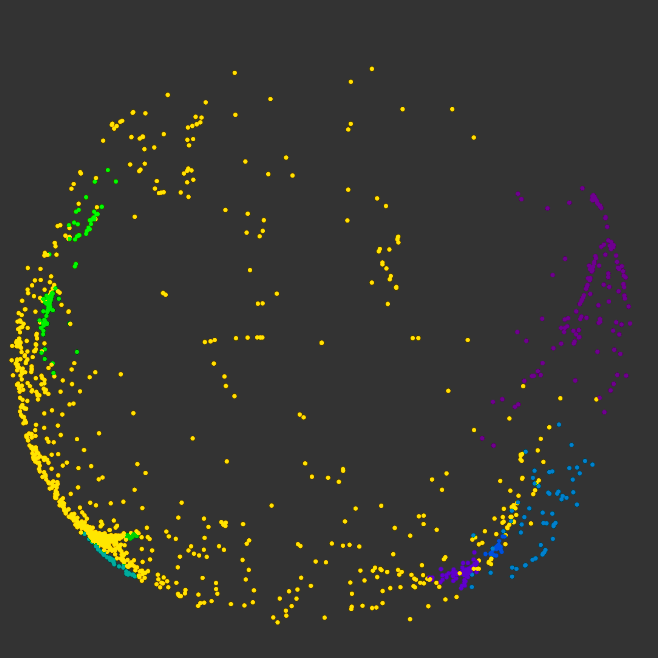
\includegraphics[width=\textwidth]{4fig/ppca.png}
         \caption{PCA}
         \label{fig:pcac}
     \end{subfigure}
     \hfill
     \begin{subfigure}[b]{0.495\textwidth}
         \centering
         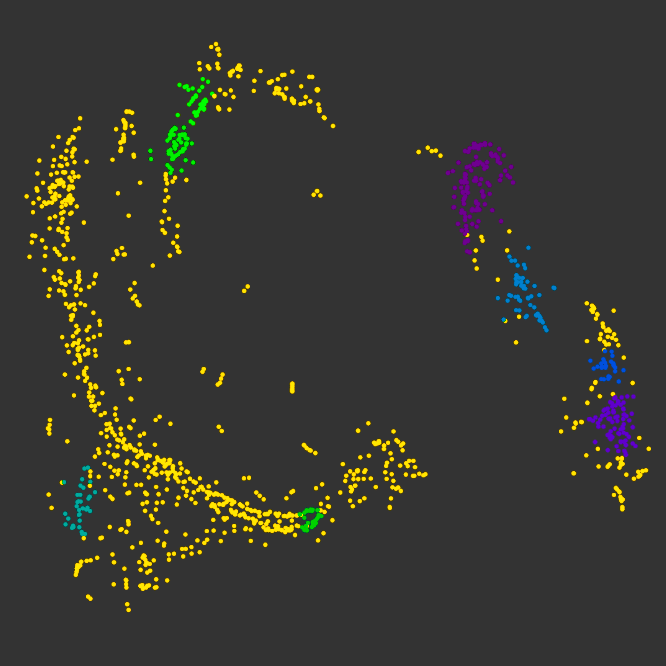
\includegraphics[width=\textwidth]{4fig/ptsne.png}
         \caption{t-SNE}
         \label{fig:tsnec}
     \end{subfigure}
     \hfill \hfill
     \begin{subfigure}[b]{\textwidth}
         \centering
         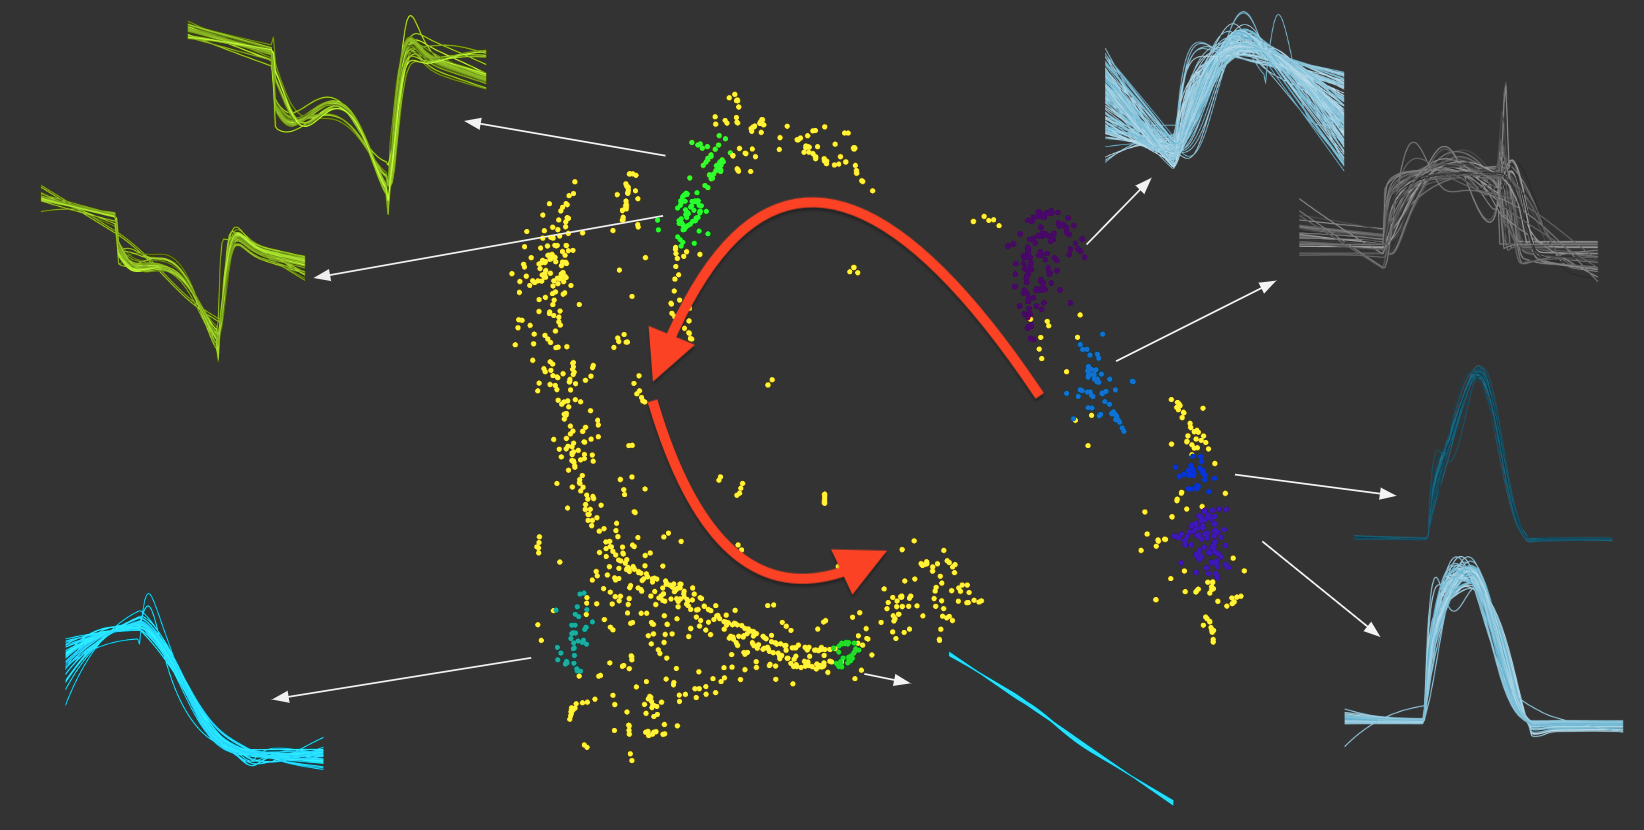
\includegraphics[width=\textwidth]{4fig/ptsneall.png}
         \caption{t-SNE with cluster outlines.}
         \label{fig:tco}
     \end{subfigure}
        \caption{\textbf{Showing the difference between PCA and t-SNE clustering.} These figures show the clustering of a set of standardized concentration profiles (c) across two styles of dimensionality reduction: PCA (a) and t-SNE (b).}
        \label{fig:threegraphs}
\end{figure}




\subsection{The Auto-Encoder (AE)}
Auto-encoders are a subclass of neural networks with primary use in compressing data (dimensionality reduction). Rather than predicting a numerical output, AutoEncoders focus on the construction and deconstruction of data through the use of an encoder and decoder pair. The encoder takes an n-dimensional input and applies a compression, reducing it to the number of dimensions in the bottleneck layer. The reduced dataset is then reconstructed within the decoder. Such a process not only allows for an easy understanding of the error of the reduced data but can also be used in the filtration of noisy or pixelated data \citep{aenoise,aeim} and as an input to more complex machine learning models.\


\begin{figure}[H]
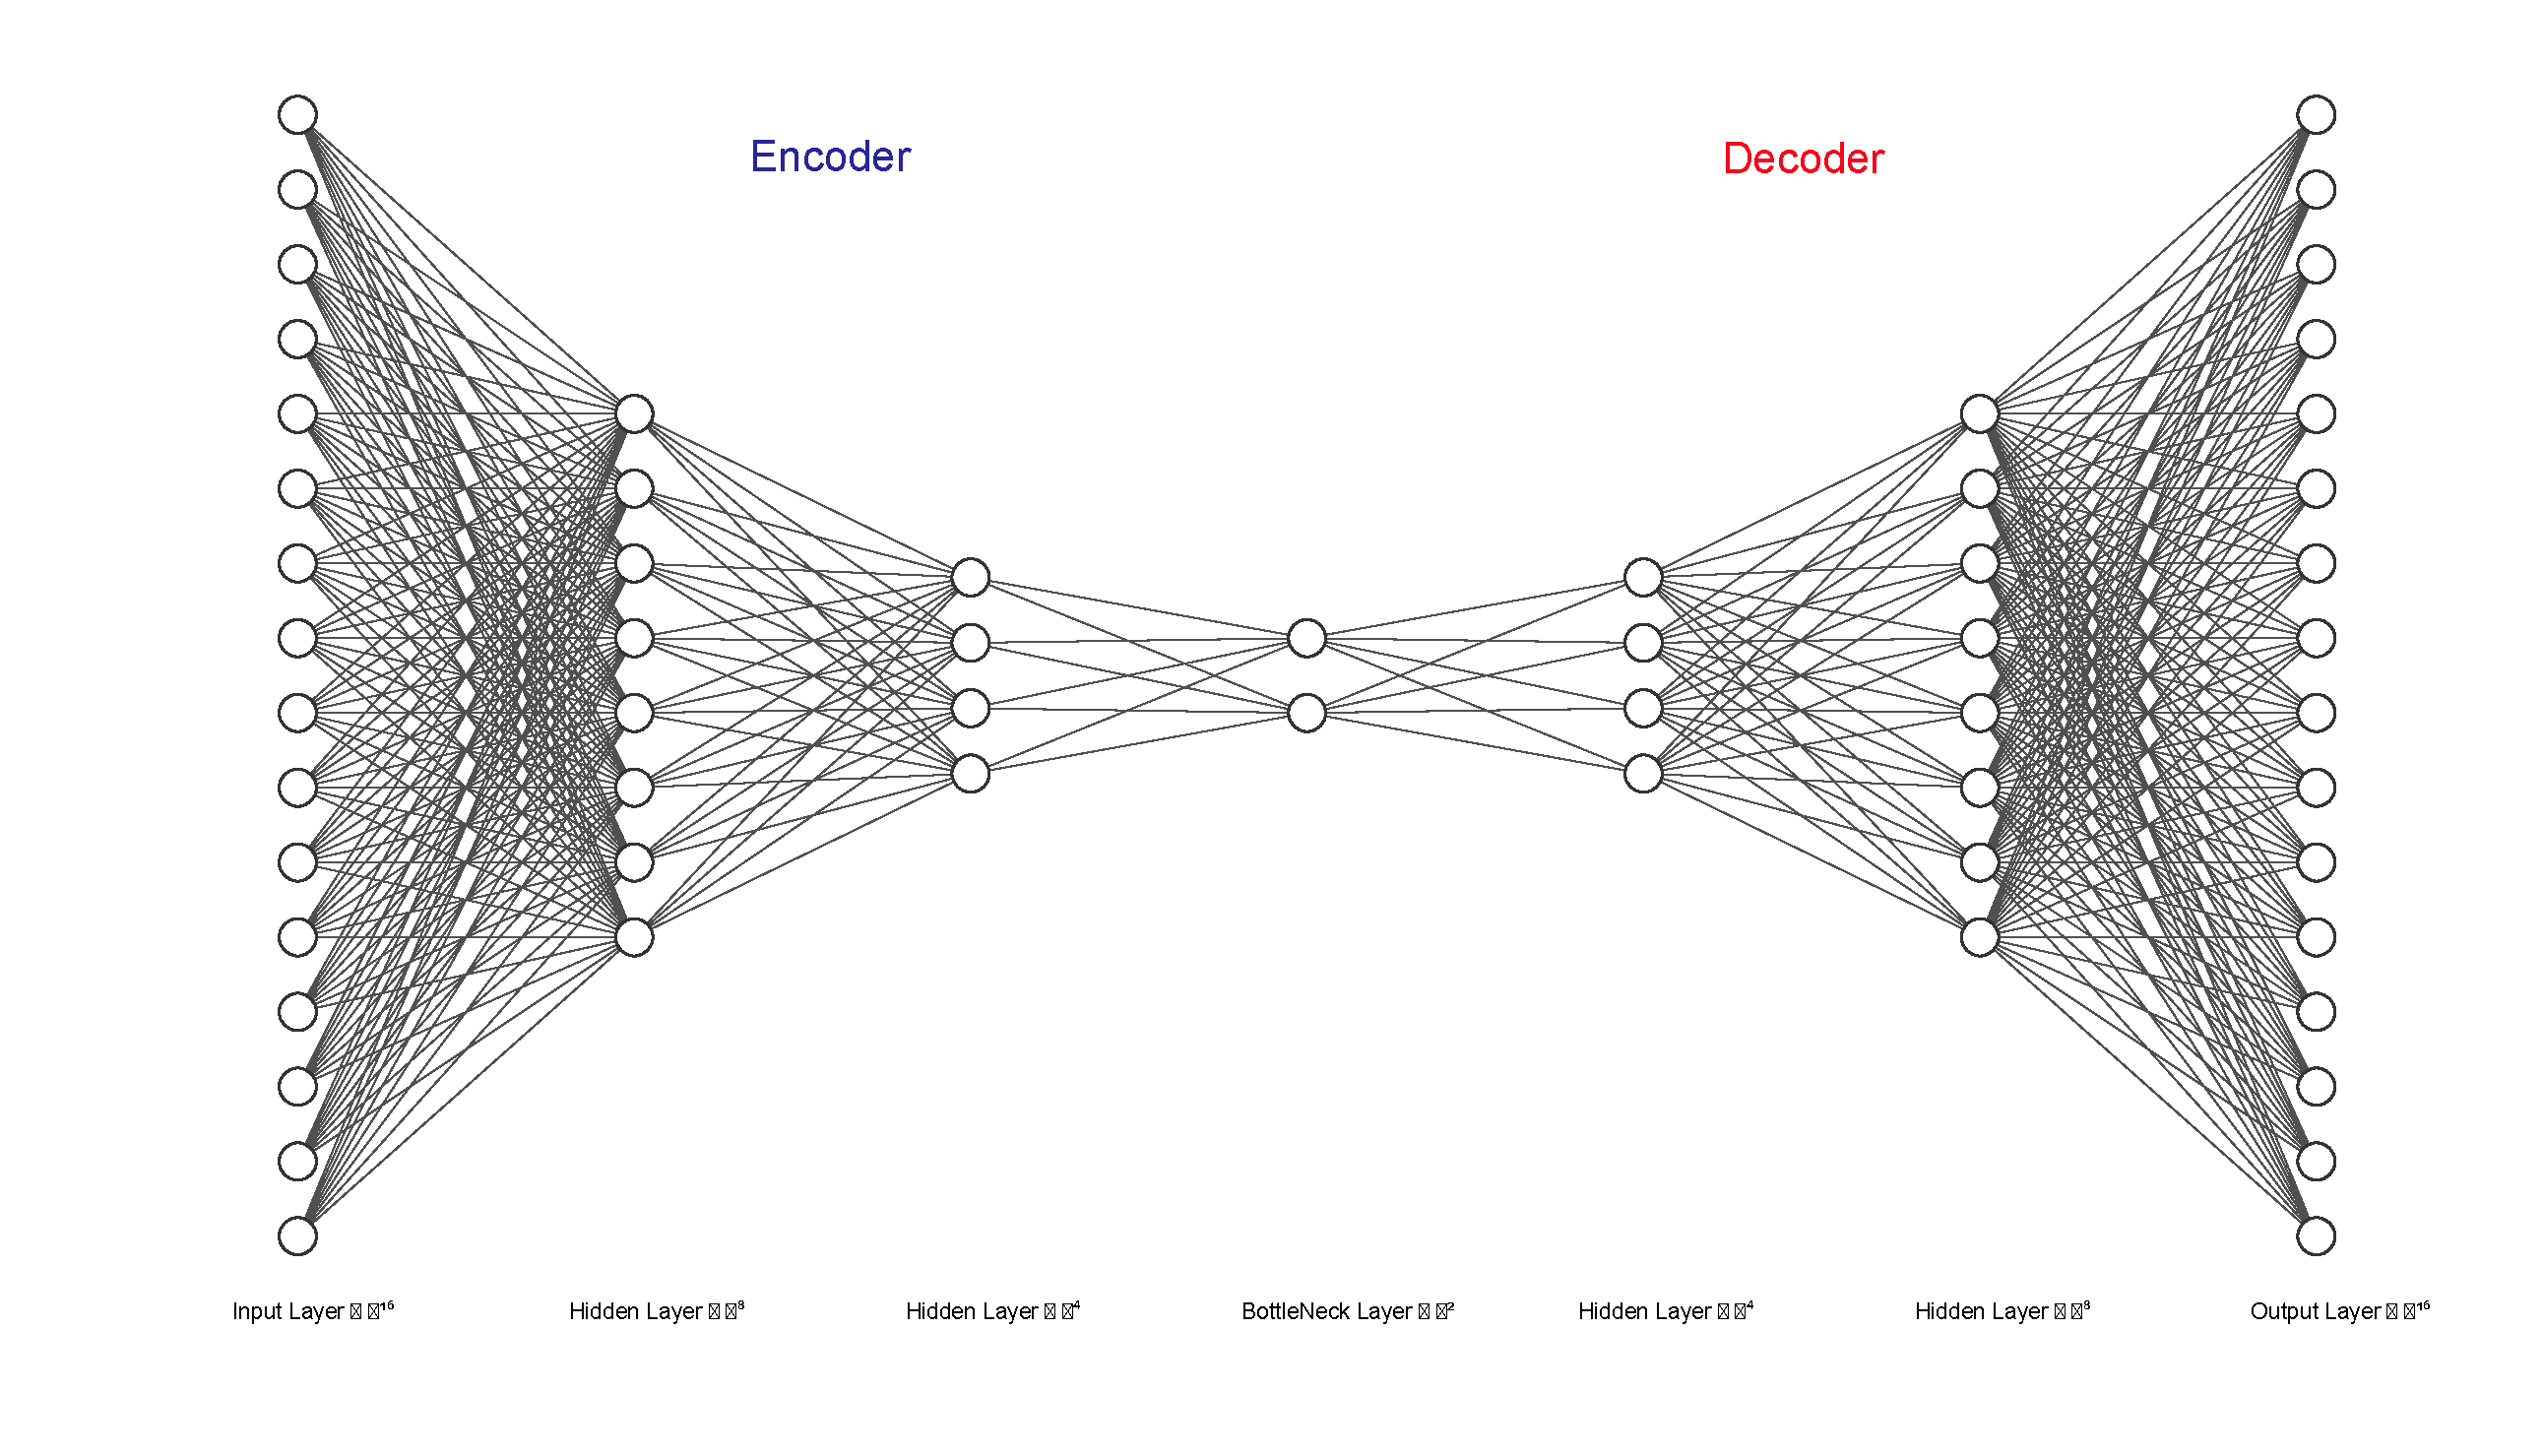
\includegraphics[width=\textwidth]{4fig/ae.pdf}
\caption{An example autoencoder structure which reduces a 16 dimentional input to 2. Draw with the aid of \citep{drawae}}
\end{figure}



There are two features of an autoencoder that make it powerful. The first is the ability to sample your latent space using the decoder. The implications of this are that we can establish features that correspond to gaps between our data points - which can have its application if the data used is sparse or incomplete. Next comes the inherent non-linearity of the model. As an autoencoder is just a neural network, the amount of information passed through each link between layers is governed by an activation function. Should this activation function be linear, the reduced dimension will be much akin to a PCA decomposition. Where PCA reduces the dimensions of a dataset by discarding those with a little effect on the variance, an autoencoder opts to combine it- here the entirety of the dataset remains encoded within the links of the AE network. To decide how data flows along the edges of the network, a series of threshold (activation) functions are used for each layer. These are described in \autoref{appendix:activation}.



\subsubsection{Demonstration of non-linear activation functions}

To demonstrate the effect of these we take a sample isopleth of Methane and Ozone, reduce it to two dimensions. This is then reconstructed back into three dimensions using the DR algorithms. 
\autoref{fig:aeiso} shows the difference between the original dataset (\autoref{fig:iorig}) and that of the PCA (\autoref{fig:ipca}) and AutoEncoder (\autoref{fig:iae}) reconstructions. Here we see a loss in the non-linearity of the original data for the PCA reconstruction. However, the use of a non-linear (tanh) activation function within AutoEncoder produces a result much closer to the original. Use of a linear activation function, however, produces a similar result to the PCA algorithm. 

\begin{figure}[H]
\begin{subfigure}{.33\textwidth}
  \centering
  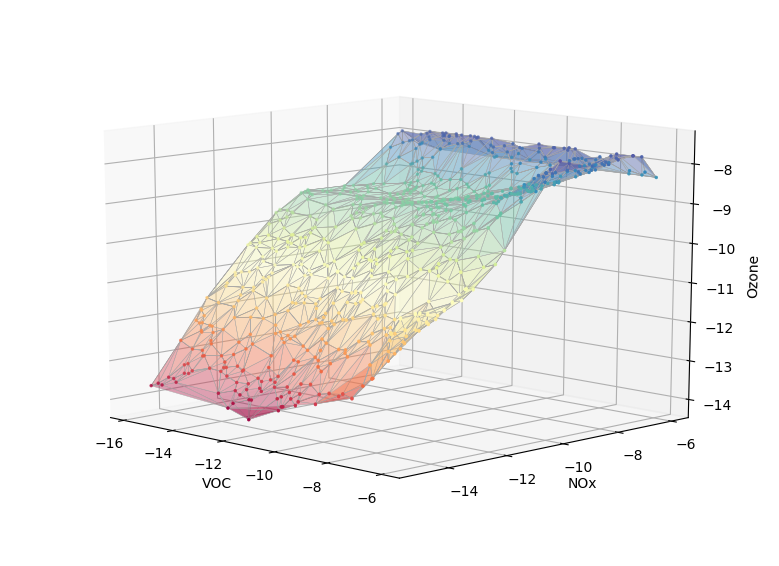
\includegraphics[width=\textwidth]{4fig/original.png}
  \label{fig:iorig}
  \caption{Original}
\end{subfigure}%
\begin{subfigure}{.33\textwidth}
  \centering
  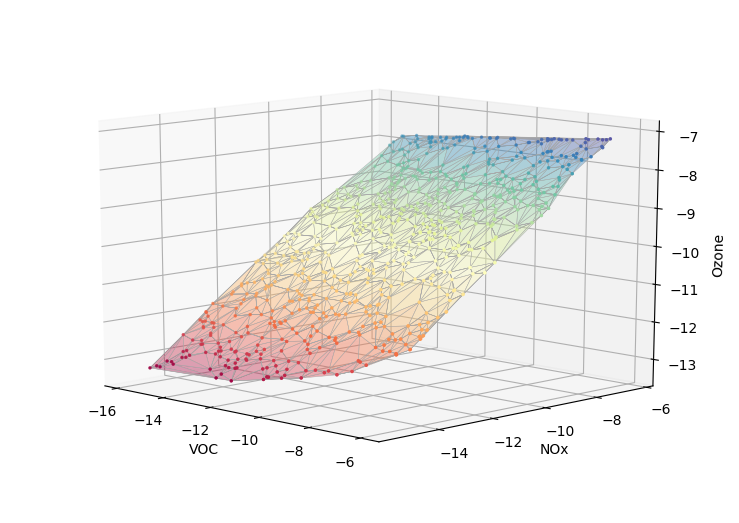
\includegraphics[width=\textwidth]{4fig/rpca.png}
  \label{fig:ipca}
  \caption{PCA}
\end{subfigure}%
\begin{subfigure}{.33\textwidth}
  \centering
  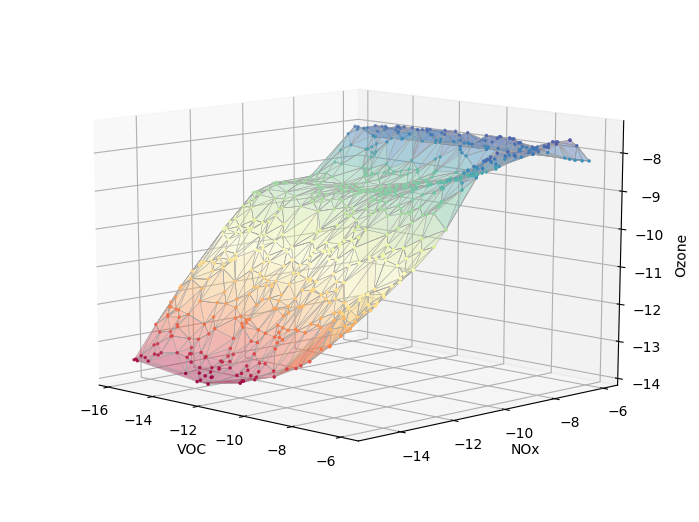
\includegraphics[width=\textwidth]{4fig/rae.png}
  \label{fig:iae}
  \caption{AE (Tanh)}
\end{subfigure}%
\caption{
\textbf{Comparing the result of the 2D encoding and decoding of an Ozone-NOx-Methane isopleth.} The original data (a) is reduced to two dimensions and then reconstructed back into 3D. This is done with Principal Component Analysis (b) and an AutoEncoder (c). The original isopleth is created using  300 simulations of different 
 intial conditions: NOx (variable), Methane (variable) and Ozone (constant). These were designed using a latin hypercube and converted into a surface plot using Delaunay triangulation. }
\label{fig:aeiso}
\end{figure}

\subsection{Node2Vec}\label{sec:n2v}
Finally, Node2Vec is an embedding algorithm designed to generate vector representations of the nodes in a \textit{undirected} and \textit{unweighted} network. Although it can be used to reduce a complex network into a 2D vector (dimensionality reduction), for this experiment we shall only use it to generate a fingerprint for a species' position within a mechanism network graph - and then apply this as an input to the DR methods above. This method of input creation has been found more computationally efficient, by circumventing the need for expensive composition, in producing better predictions on network-related tasks compared to more classical methods such as PCA \citep{node2vec}.


\begin{figure}[H]
  \centering
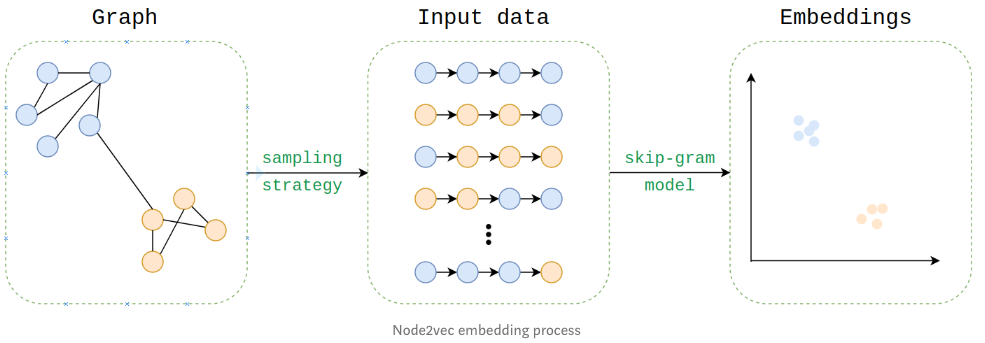
\includegraphics[width=\textwidth]{4fig/n2vproc.png}
\caption{The process of converting a graph into a vector using Node2Vec. Source:\citep{n2vimg}}\label{fig:n2vprocess}
\end{figure}


The process of converting the graph structure (\autoref{fig:n2vprocess}) into a numerical vector node embedding starts by taking a series of $2^{nd}$ order random walks. These describe the neighbourhood of a node in the form of a set of random walk paths, much in the same way words are dependant on their neighbours within a sentence: \autoref{eqn:w2varrow}.


\begin{equation}
ISOPRENE \rightarrow OH \rightarrow TISOPA \rightarrow ISOPBO_2 \rightarrow TISOPA \rightarrow...
\label{eqn:w2varrow}
\end{equation}

This methodology allowed for the use of word2vec algorithm, converting the walk into a vector (\autoref{sec:w2v})



\subsubsection{Sentence construction by sampling of a network}
The probability and path depend both on a set of arguments and a random seed provided to the model. The return and input parameters ($p\ \&\ q$) determine how fast we explore the network and our probability to leave the neighbourhood, \autoref{fig:n2vedge}. In a system, where the previous path is from $t$ to $v$, we may calculate the probability of returning to $t$ as $1/p$, going to a mutual node connected between $t$ and $v$ as 1, and viewing a new node as $1/q$.
If $q>1$ we have a high probability to end up at nodes close to $t$, and with $q<1$ we are likely to explore other nodes. Additionally if we chose $p> \max{q,1}$ we are less likely to return to an already visited node ($p < \min{q,1}$ is likely to generate a backwards step). Since we wish to generate a `local' view, but do not wish to return to $t$ we select  $q \ge 1$ and $p > q$ our parameters as  $p = 2.0,q=1.1$.  In the case of a weighted graph (something that we are \textit{not} exploring within this chapter) the resultant $alpha$ value calculated is further multiplied by the edge weight.

To run the simulation, we use the python2 code provided by the original paper \citep{node2vec} with a set of 50000 random walks, each of length 9. The reasoning behind this is that we have a large graph, with a power-law like structure (where species are often heavily connected, \autoref{ch3}).

\textit{NOTE: This process takes over a week to compute (in serial), and then the binary file containing all walks in character form approaches 10 GB, for the complete MCM. }

\begin{figure}[H]
  \centering
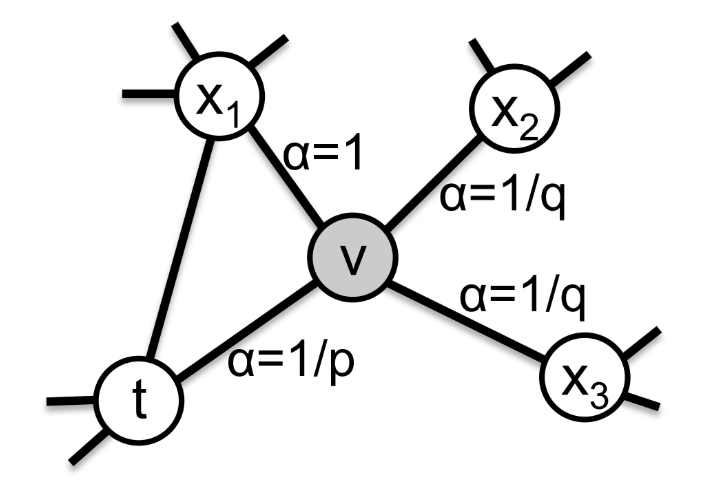
\includegraphics[width=0.5\textwidth]{4fig/n2vedge.png}
\caption{Calculation of the random walk path. Source:\citep{node2vec}}\label{fig:n2vedge}
\end{figure}



\subsubsection{Word2Vec}\label{sec:w2v}
Once we have constructed our random path `sentences' (e.g. \autoref{eqn:w2varrow}), we can make use of Googles word2vec algorithm \citep{w2v}. This is similar to an auto-encoder in many regards; however, the algorithm looks at neighbouring words (or species) in the corpus rather than learning word embeddings using reconstruction. This form of representation has found many uses beyond the realm of natural language processing. Some of these are objects, people, code, tiles,genes and graphs \citep{objects,people,code,tile,gene,graph2vec}.


% 
% https://skymind.ai/wiki/word2vec
% http://mccormickml.com/2016/04/19/word2vec-tutorial-the-skip-gram-model/
% 

\subsection{Summary}
There exist several methods of reducing a complex dataset into a smaller one. PCA is the simplest method to understand but is constrained to linear decompositions. AutoEncoders can have both a linear and non-linear response, based on the activation functions that they use, and t-SNE applies a non-linear grouping which mimics a complete force-directed graph. 

Having defined each method, we next explain how they will be evaluated (\autoref{sec:drvis}), before applying them to the MCM in \autoref{eqn:w2varrow}.




\section{Visualisation of clustering}\label{sec:drvis}

In assessing the validity of clustered space, we require a level of exploratory data analysis. To reveal features of interest, we plot the reduced 2D dataset and apply interactivity coupled with a selection of visualisation techniques described below. This section outlines the different visualisation methods which are used.

\subsection{Viewing the 2D species embeddings}
Since the different DR algorithms return data on various scales, comparison between the outputs is not straightforward. To overcome this outputs in $x$ and $y$ are normalised (scaled between \{0,1\}), before being plotted as a scatterplot. 


\subsection{Exposing overlapping data}
If the nodes within a tight-knit cluster overlap, this can cause obfuscate the results and limit the user's ability to select them. As an initial test, node sizes can be reduced. However, this may often result in points too small to pick. The other solution which was used is to create a force-directed graph where each point is strongly attracted to their initial position. Here we can apply collision detection, while still preserving the overall grouping of nodes within a cluster - a technique that was seen in \autoref{ch4}.


\subsection{Gooey Effect (Gaussian Blur)}
Taking a quote from \cite{lessmore}:
\emph{``The more stuff in it, the busier the work of art, the worse it is. More is less. Less is more. %The eye is a menace to clear sight. 
''} and combining it with the work from \autoref{ch1}, we realise that showing each species, when observing overall clusters just add unnecessary clutter to the images. Instead, since we are only interested in the clusters as a unit, a `gooey effect' filter can be applied. This works by merging nearby points into a single water-like blob using a gaussian blur\footnote{Here a gaussian blur of standard deviation 3.7 and a colour matrix [1 0 0 0 0  0 1 0 0 0  0 0 1 0 0  0 0 0 37 -5] is used.}. Here since each point is allocated a colour, if a colour gradient exists, then there are multiple clusters occupying the same place. The aim of this is to reduce the cognitive load on the end-user by reducing the number of distinct objects that they need to take in.



\subsection{Four Colours Theorem}\label{sec:4col}
When plotted, the number of clusters detected often exceeds the number of categorical colours available. In cartography, it has been noted that the colouring of neighbouring polygons should at most take four colours. This is the origin of the four colours theorem \cite{fourcolour}, of which a greedy implementation is applied.

The aim of this is to show item boundaries (for instance countries, or in our case clusters) while reducing ambiguity (if, say, two neighbours have the same colour). The algorithm I adapted uses the Delaunay tesselation scripts contained within DataDrivenDocuments.js (d3js) \cite{d3js}. This partitions our plane into polygon-regions, each of which includes boundaries at the furthest distance from each point (Voronoi cells) \cite{delaunay}. First, we chose a random cell and assign it a colour. 
Next, all its neighbours are recursively iterated, giving them the lowest possible colour in a list, which does not match any of their neighbours. Although such a greedy approach does not produce an optimum result, it allows for the colouring of data with $\le 5$ distinct colours, as is shown in \autoref{fig:4col}.


\begin{figure}[H]
  \centering
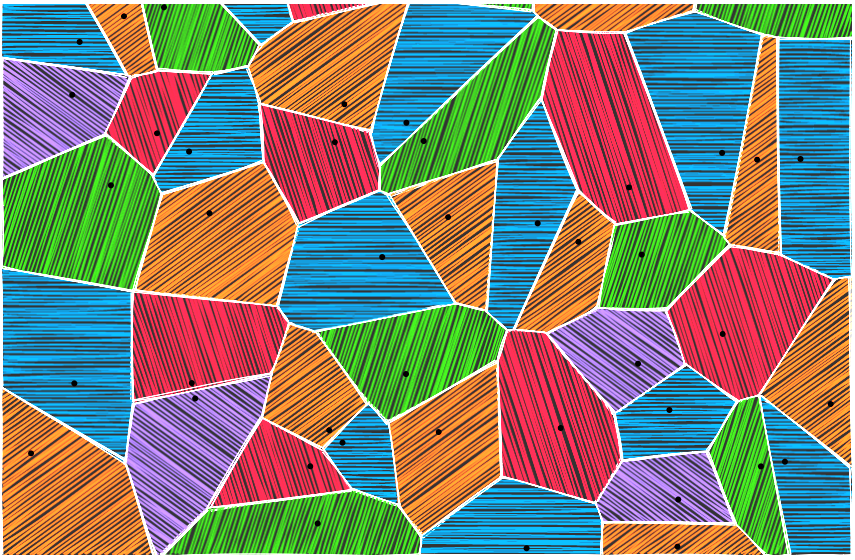
\includegraphics[width=.8\textwidth]{4fig/4col.png}
\caption{\textbf{An example 4 colour matching} This uses the first implementation of the algorithm mentioned in \autoref{sec:4col}. The greedy approach does not often find the optimum solution, which may result in 5 colours instead. Observable Notebook : \cite{4colobs}}\label{fig:4col}
\end{figure}


Having defined all the visualisation techniques we move on to explain the clustering algorithms which are used, and how `goodness of fit' may be measured in the clustering context.

%%%%%%%%%%%%%%%%%%%
%%%%%%%%%%%%%%%%%%%

\section{Cluster Evaluation}
The previous section discussed methods of visualising the reduced data for use with interactive exploratory data analysis. In this section we look at the use of vector clustering algorithms\footnote{Vector clustering is the grouping of data based on their proximity or density to other nearby points} (\autoref{sec:drclustt}) to highlight groups in a 2D dataset, as well an automated method of assessing the quality of the clusters selected (\autoref{sec:silo}) and feature extraction (\autoref{sec:drfeature}).



\subsection{Automated selection of clusters}\label{sec:drclustt}
    When it comes to clustering data points in a dataset, there exist a range of methods which may accomplish a task, \autoref{fig:clustereval}. Most often, the k-means \citep{kmeans}, is used as it is fast and straightforward to understand. However, its linear method of partitioning cannot capture the splits between non-linear relationships of real data. The other problem is that an estimate for the number of expected clusters is required - something that is often unknown without prior understanding of the data. When this is the case, often it is easier to select the nodes with interactivity manually.

In contrast, density-based clustering techniques such as GMM (\citep{scikit}) or DBSCAN (\citep{DBSCAN}) tend to be better at locating non-linear trends in the data. The DBSCAN algorithm asses the distribution of data across a specific location. This allows clusters with a high density of datapoints to be located without the need for a predefined number as an input. Another method: OPTICS (Ordering Points To Identify the Clustering Structure) \citep{optics}, shall be used\footnote{ If using Python 2, the library for this needs to be extracted from the sci-kit-learn library for python3 package and altered to run with the previous version. (See copy in attached code.)}. This is an adaptation of the DBSCAN algorithm which does not require the specification of a minimum distance between points (for the density estimate)- instead, we specify a gradient for the distribution and the minimum number of points for a cluster to be classified.


\begin{figure}[H]
     \centering

         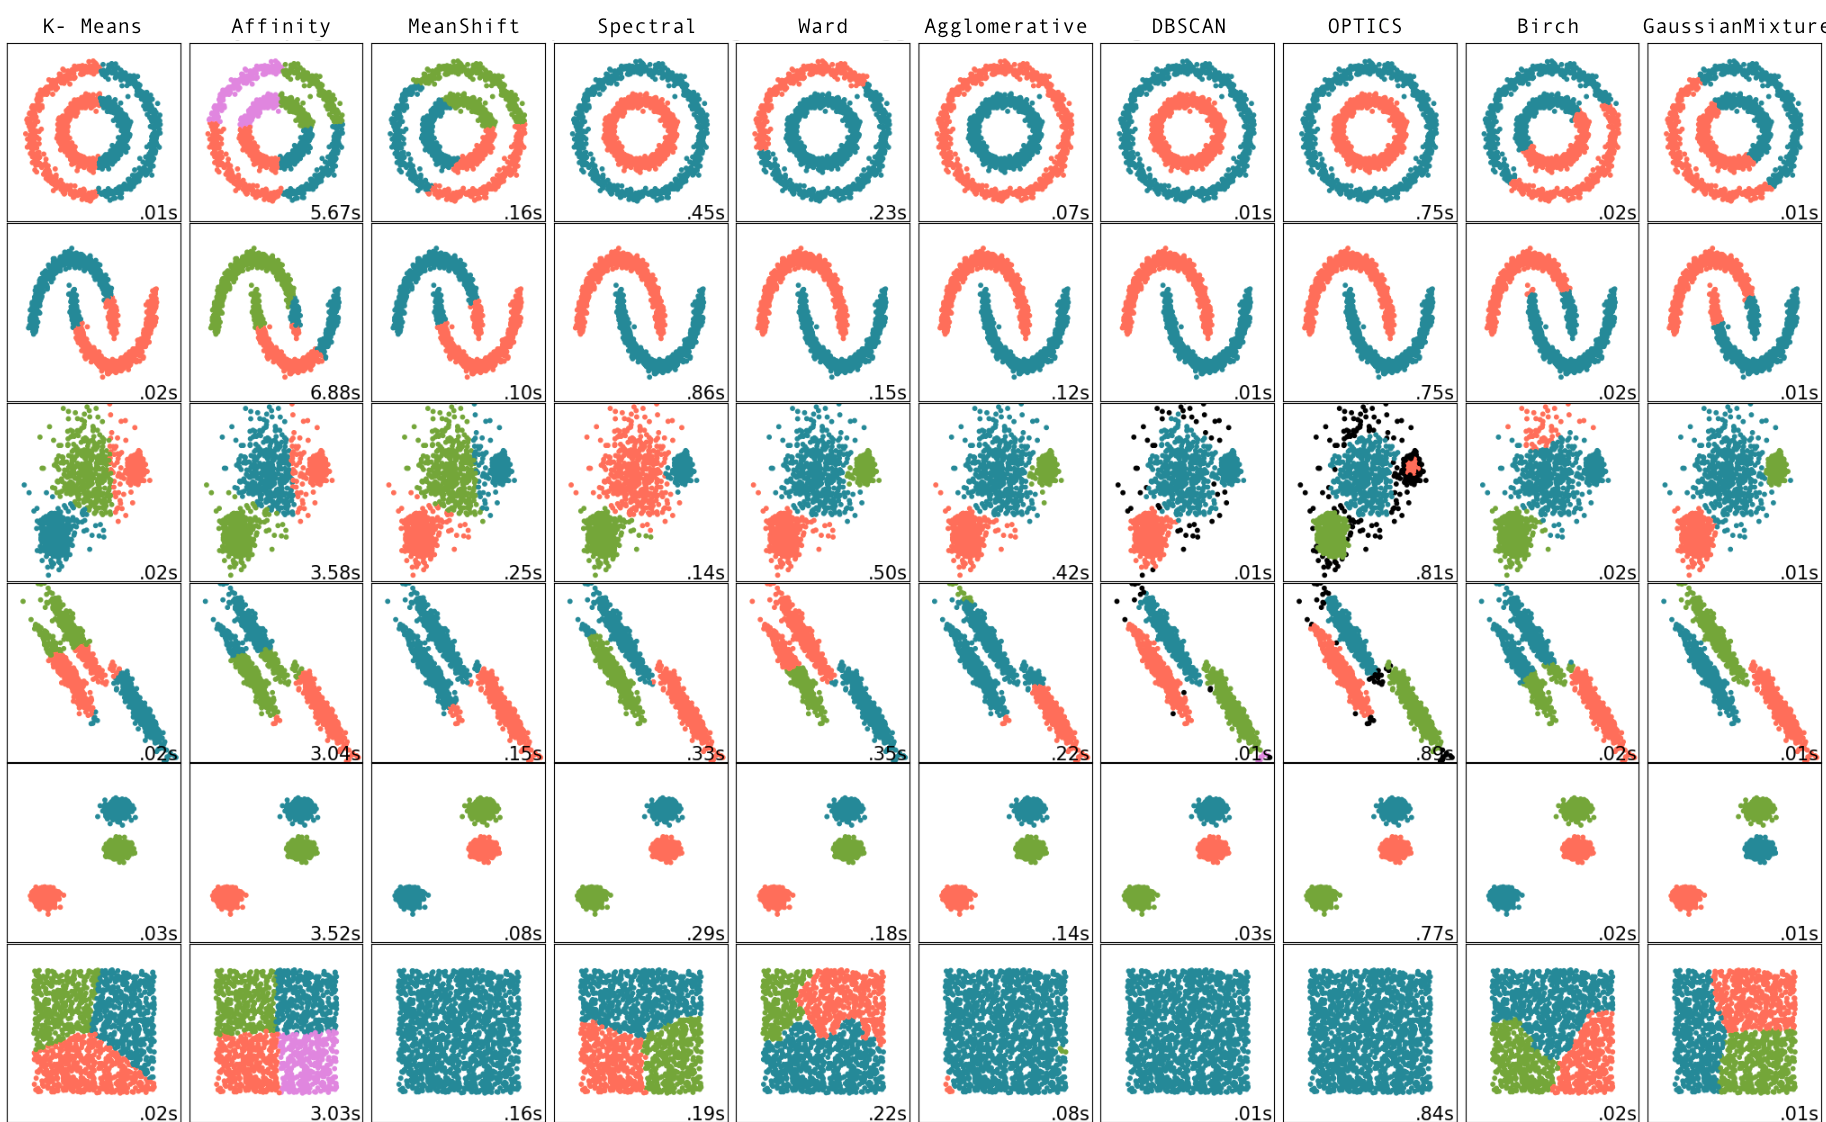
\includegraphics[width=\textwidth]{4fig/clustereval.png}

        \caption{\textbf{A comparison of different clustering methods on a toy dataset.} The plot shows the performance of several vector clustering algorithms in Scikit-Learn. Cluster algorithms are represented across the horizontal axis and several types of datasets are across the vertical. Clustered groups are coloured. Source: \cite{clustereval}}
        \label{fig:clustereval}
\end{figure}


When deciding which algorithms to use, each algorithms' ability to partition non-linear data is considered. 
The first two rows of \autoref{fig:clustereval} show data which cannot be partitioned linearly, here spectral, DBSCAN and optics are the only clustering algorithms to identify both correctly. It is for this reason that we shall look at these for the remainder of the chapter. 

In selecting a value for the results section, several clustering algorithms, with a wide range of input parameters, are run. From these, the simulation with the best silhouette coefficient (\autoref{sec:silo}) is taken. 




\subsubsection{Clustering (Silhouette) coefficient}\label{sec:silo}
The silhouette measure is a tool used for acessing the validity of a set of clusters. Here each cluster is represented as a silhouette, based on the comparison of its tightness and separation. To calculate the silhoette coefficient we look at the intra-cluster $a$ and the mean inter-cluster\footnote{Inside and between different clusters.} distance $b$. The silhouette cluster can then be described using \ref{silhouette,sklearn}:

\begin{equation}
s(i) = \frac{b(i)-a(i)}{\max{ a(i), b(i)}}
\end{equation}

This gives a value $-1 \le s(i) \le 1$. Values near zero suggest overlapping clusters, 1 - dense, well-separated clusters and negative values indicate that a sample may have been incorrectly classified. In using this method, we can get an overview of how well individual objects lie within their assigned cluster.




\subsection{Feature Extraction}\label{sec:drfeature}
Upon establishing a set of DR datasets, and their groups (the clusters of species they contain), it is important to evaluate what input features they represent. Rather than doing this manually we make use of Random Forests - described below.

\subsubsection{Random Forrests}
Random forests \citep{rfrr}, are a subset of ML algorithms called ensemble learning. This means that they train a large number of decision trees, each on a random subset of the original features. A decision tree is a tree formed from a series of conditionals\footnote{Questions with a True/False answer}, much like a perceptron network (\autoref{sec:perceptron}) with binary activation functions. Random forests introduce a level of additional randomness by selecting only a subset on which to create each decision tree. This may introduce a higher bias, but lowers the overall model variance, which creates a better (more robust) model. Such methods have been applied to replacing the computationally expensive process of chemistry integration of GEOS-Chem (a global 3D model of tropospheric chemistry) \citep{geosrf} and the prediction of global sea-surface iodine based on observations coupled with sea-surface temperature, depth, and salinity \citep{iodene}.

\subsubsection{Calculating importance using Random Forrests}
Since random forests are in essence a collection of decision trees, it is possible to generate a `decision tree aggregate' to visualise the ensemble structure of the random forest \citep{forrester} (\autoref{fig:iodenetree}). Alternatively, if all that is required is the relative importance of each feature, the RandomForrestClassifier from \cite{sklearn} provides a quick and easy way of understanding which features matter, 
\citep{handsonml}. This works by aggregating the weighted nodes which use a certain feature using the number of samples and then scales the result to 1. We use this method to access the overall importance of features within each DR output and identify the differences between clusters.
%bagging an aggregate collection of TreeS


\begin{figure}[H]
     \centering
         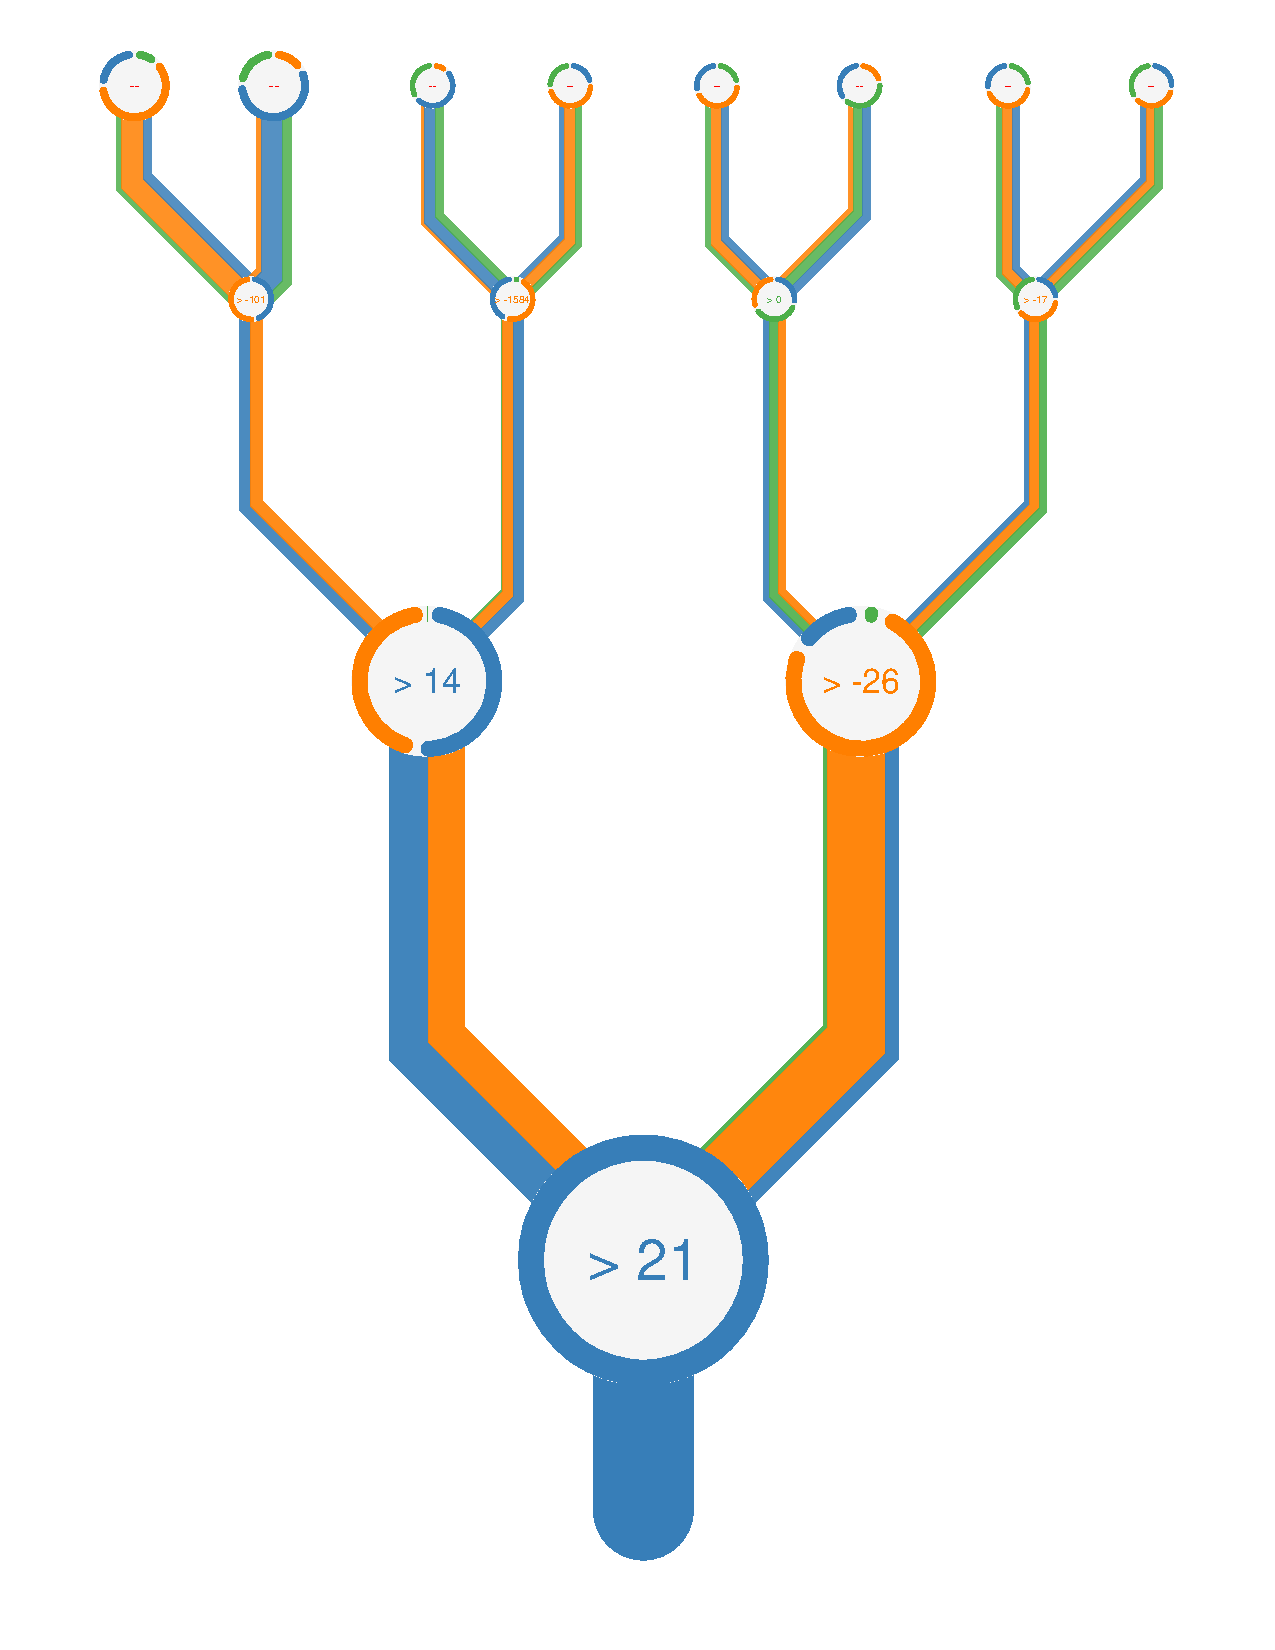
\includegraphics[width=.55\textwidth]{4fig/Oi_prj_features_of_RFR(TEMP+DEPTH+ChlrA)_for_depth_5_white.pdf}
        \caption{\textbf{A decision tree aggrogate from a random forrest plotted with the Epiphyte version of the TreeSurgeon program \citep{forrester}.} The data originates from \cite{iodene} and the imporance of Tempearature (blue), Depth (orange) and Chlorophyll $a$ (green).}
        \label{fig:iodenetree}
\end{figure}


% 
% Random Forrest Classifier from sklearn, top n features.
% https://github.com/MaartenGr/CustomerSegmentation/blob/master/Customer%20Segmentation.ipynb
% https://www.ncbi.nlm.nih.gov/pmc/articles/PMC5732374/

\textit{NOTE: The only downside is that Random Forrests are in themselves ML techniques which also need to be evaluated. To do this, as they are simply being used as indicators of cluster properties which we are to explore further, we can initiate a collection of 300 random Forrest classifiers, from which we take the median. A sort of ensemble learning from an ensemble. }


\section{Results}\label{sec:drres}
% 
There exist many methods to define the chemical structure of the species within the MCM. In this section, we attempt to evaluate their effectiveness for exhibiting the defining functional groups and characteristics used for constructing the mechanism. First, we explore the distribution of clusters and the ability of different DR algorithms to visually separate various groups of chemistry (\autoref{sec:cldist}). Next, the functional groups (taken from the MCM development protocol) are explored within each DR algorithm (\autoref{sec:fsclust}). Finally, a selected example for each DR method is taken and explored in further detail (\autoref{sec:selectcomp}).

\subsection{Cluster distribution}\label{sec:cldist}

Start with the visual comparison and compare it with the silhouette values. 




\paragraph*{Principle Component Analysis}


\begin{table}[H]
    \centering
        \subimport{tables/}{silhouettepca.tex}
        \caption{The inputs to the PCA dimensionality reduction algorithm sorted by the best obtained silhoette coefficient.  }
        \label{tab:pcasil}
\end{table}



\begin{landscape}
\begin{figure}[H]
    \subimport{tables/}{pcadr.tex}
    \caption{\textbf{Comparing clusters for all inputs after a reduction to 2 dimensions using Principle Component analysis.}
    Each graph has undergone several clustering algorithms under a range of parameters. The result with the best silhouette coefficient has been chosen. Colours follow the greedy four colour theorem and are there only to indicate the contrast between cluster boundaries.}
    \label{fig:pcavis}
\end{figure}
\end{landscape}






\paragraph*{Auto Encoder Encoding}

\begin{table}[H]
    \centering
        \subimport{tables/}{silhouetteae.tex}
        \caption{The inputs to the AutoEncoder dimensionality reduction algorithm sorted by the best obtained silhoette coefficient.  }
        \label{tab:aesil}
\end{table}





\begin{landscape}
\begin{figure}[H]
    \subimport{tables/}{aedr.tex}
    \caption{\textbf{Comparing clusters for all inputs after a reduction to 2 dimensions using an AutoEncoder.}
    Each graph has undergone several clustering algorithms under a range of parameters. The result with the best silhouette coefficient has been chosen. Colours follow the greedy four colour theorem and are there only to indicate the contrast between cluster boundaries.}
    \label{fig:aevis}
\end{figure}
\end{landscape}




\paragraph*{t-Distributed Stochastic Neighbor Embedding}

\begin{table}[H]
    \centering
        \subimport{tables/}{silhouettetsne.tex}
        \caption{The inputs to the t-SNE dimensionality reduction algorithm sorted by the best obtained silhoette coefficient.  }
        \label{tab:tsnesil}
\end{table}




\begin{landscape}
\begin{figure}[H]
    \subimport{tables/}{tsnedr.tex}
    \caption{\textbf{Comparing clusters for all inputs after a reduction to 2 dimensions using t-SNE.}
    Each graph has undergone several clustering algorithms under a range of parameters. The result with the best silhouette coefficient has been chosen. Colours follow the greedy four colour theorem and are there only to indicate the contrast between cluster boundaries.}
    \label{fig:tsnevis}
\end{figure}
\end{landscape}



\subsection{Feature selection comparison}\label{sec:fsclust}

\begin{figure}[H]
    \subimport{tables/}{pcalegend.tex}
    \caption{\textbf{Comparing feature importance for PCA clusters.}}
    \label{fig:pcalegend}
\end{figure}


\begin{figure}[H]
    \subimport{tables/}{aelegend.tex}
    \caption{\textbf{Comparing feature importance for AE clusters.}}
    \label{fig:aelegend}
\end{figure}
\begin{figure}[H]
    \subimport{tables/}{tsnelegend.tex}
    \caption{\textbf{Comparing feature importance for t-SNE clusters.}}
    \label{fig:tsnelegend}
\end{figure}


\subsection{Individual Cluster Comparison}\label{sec:selectcomp}